  \documentclass{article}
\usepackage{multicol} %multiple columns
\usepackage{amsmath,amsthm,amssymb,amsfonts} 
\usepackage[margin=0.5in]{geometry} %0.5 in margins
\usepackage{gensymb} %degree symbol \degree
\usepackage{empheq} %box multiple equations
\usepackage{float} %placing image HERE
\usepackage{tikz}
\usepackage{physics}
\usepackage{hyperref}
\hypersetup{
    colorlinks=true,
    linkcolor=red,
    filecolor=magenta,      
    urlcolor=cyan,
    pdftitle={Overleaf Example},
    pdfpagemode=FullScreen,
    }

\title{PUEC 2022}
\author{Team \textbf{AceD}\\
Matthew Chen, Ashmit Dutta, Bhanu Narra, Peter Xu}
\date{\today}

\newcommand{\ode}[2]{\ensuremath{\frac{\mathrm{d}#1}{\mathrm{d}#2}}}
\newcommand{\pde}[2]{\ensuremath{%
		\frac{\partial #1}{\partial #2}}}
%usage: \pde{y}{x} will output dy/dx

\newcommand{\oden}[3]{\ensuremath{\frac{\mathrm{d}^{#1}#2}{\mathrm{d}{#3}^{#1}}}}
\newcommand{\pden}[3]{\ensuremath{\frac{\partial^{#1}#2}{\partial{#3}^{#1}}}}
\newcommand*\widefbox[1]{\fbox{\hspace{2em}#1\hspace{2em}}}

%\numberwithin{equation}{chapter} %equation numbering: (chapter).(#eq in that chapter)
%\setcounter{tocdepth}{0} %only display parts and chapters in the table of contents, 

\newenvironment{amatrix}[1]{%
	\left(\begin{array}{@{}*{#1}{c}|c@{}}
	}{%
	\end{array}\right)
}
%\begin{amatrix}{2} 	1 & 2 & 3 \\  a & b & c		\end{amatrix} 
% will output a 3x2 matrix with a vertical line between the 2nd and 3rd column 
\usepackage[utf8]{inputenc}
\usepackage{xcolor}

\begin{document}

\maketitle

\tableofcontents
\newpage 
We referred to several different books in this citation, namely \cite{Ryder1996Quantum}\cite{sakurai2006advanced}\cite{schwartz2014quantum}\cite{zee2010quantum}.
\section{The Classical Action}
\subsection{Exercise 1: First step}
The function $f$ changes in both $x_1$ as well as in $x_2$, so when we write the change in the function $\delta f$, we have to consider each individual change of the function in terms of $x_1$ and $x_2$. To do this, we multiply the gradient of the function $\partial f/\partial x_i$ times $x_i$ to get the change and we do this for each $x_1$ and $x_2$. Therefore, 
\begin{equation}\label{1}
\delta f = \delta x_1 \pdv{f}{x_1} + \delta x_2\pdv{f}{x_2}.
\end{equation}
\subsection{Exercise 2: Second Step}
We consider the change in action. By applying equation \eqref{1}
\begin{align}
\delta S &= \delta\left(\int_{t_a}^{t_b}L(x, \dot x, t) \dd t\right) \\
&= \int_{t_a}^{t_b}\delta L \dd t \\
&= \int_{t_a}^{t_b}\left(\delta x \pdv{L}{x} + \delta \dot{x}\pdv{L}{\dot x}\right)\dd t.
\end{align}
We can apply integration by parts to the second term. Using the below formula
\begin{equation}
    \int u\dd v = uv - \int v \dd u,
\end{equation}
we say that $u = \pdv{L}{\dot x}$ and $v = \dot x$. Hence, 
\begin{equation}
    \delta S = \left.\delta x\pdv{L}{\dot x}\right|_{t_a}^{t_b} + \int_{t_a}^{t_b}\delta x\left(\pdv{L}{x} - \dv{}{t}\left(\pdv{L}{\dot x}\right)\right)\dd t.
\end{equation}
Note that the first term vanishes as $\delta x(t_a) = \delta x (t_b) = 0$. We want action to minimized, so $\delta S = 0$ which means 
\begin{equation}\label{EL}
    \pdv{L}{x} - \dv{}{t}\left(\pdv{L}{\dot x}\right) = 0.
\end{equation}
\subsection{Exercise}
The lagrangian is $L$ = Kinetic energy - Potential energy. Assuming a point of reference where the potential energy is $U(x)$, we can say the lagrangian consists of only kinetic energy, or 
\begin{equation}\label{2}
    L = \frac{1}{2}m\dot x^2 - U(x)
\end{equation}
From equation \eqref{2} and equation \eqref{EL}, we have
\begin{equation}\pdv{}{x}\left[\frac{1}{2}m\dot x^2 - U(x)\right] - \dv{}{t}\left(\pdv{}{\dot x} \left[\frac{1}{2}m\dot x^2 - U(x)\right]\right) = 0.\end{equation}
The first term becomes $\partial U/\partial x$ because kinetic energy is only dependant on $\dot x$ and potential energy is dependant on $x$. Similarly, the second term becomes $m \ddot x$ for the same reasons. Hence, we finally yield
\begin{equation}
    -\pdv{U(x)}{x} = m \ddot x
\end{equation}
As the negative gradient of potential energy is force and $\ddot x = a$, we yield 
\begin{equation}
    F = ma.
\end{equation}
\subsection{Exercise}
If there is no external force, then we say that the potential energy is 0 as the negative gradient results in force. So, we consider the action of only the kinetic energy component. 
\begin{equation}
    S = \int_{t_a}^{t_b}\frac{1}{2}m\dot x^2 \dd t = \frac{1}{2}m\frac{(x_b - x_a)^2}{t_b - t_a}.
\end{equation}
\subsection{Exercise}
We consider the change of the hamiltonian with respect to time. If it is equal to zero, then the Hamiltonian does not change and the potential energy does not change on velocity or time explicitly. 
\begin{equation}
    \dv{H}{t} = \ddot{x}\pdv{L}{\dot x} + \dot x \dv{}{t}\left(\pdv{L}{\dot x}\right) - \dv{L}{t}.
\end{equation}
We know that the change in lagrangian with respect to time is zero, so the third term vanishes. By equation \eqref{EL}, the first two terms vanish since:
\begin{equation}
    \pdv{L}{x} - \dv{}{t}\left(\pdv{L}{\dot x}\right) = 0 \to \dot x \pdv{L}{x} - \dot x \dv{}{t}\left(\pdv{L}{\dot x}\right) \to \ddot x \pdv{L}{\dot x} - \dot x \dv{}{t}\left(\pdv{L}{\dot x}\right) = 0
\end{equation}Hence, 
\begin{equation}
    \dv{H}{t} = 0
\end{equation}
and our statement is proven. If the potential energy does not depend on $\dot x$, then $\partial L/\partial \dot x$ is only dependent on kinetic energy $T$. As $T = \frac{1}{2}m \dot x^2$, then $\dot x (\partial L/\partial \dot x) = \dot x (m \dot x) = m \dot x^2$. Hence, the Hamiltonian can be rewritten as 
\begin{equation}
    H = m \dot x^2 - \frac{1}{2}m \dot x^2 + V(x) = \frac{p^2}{2m} + V(x).
\end{equation}
\newpage 
\section{Path-integral in Quantum Mechanics}
\subsection{Exercise}
We know that the action is given as
\begin{equation}
    S = \int_{t_a}^{t_b}L(x, \dot x, t) \dd t = \lim_{\Delta t\to 0}\sum L \Delta t
\end{equation}
The lagrangian has units of energy as it is given as the difference of kinetic and potential energies. Therefore, the action has units of Energy $\times$ time. Planck used $\hbar$ when describing the blackbody spectrum. The energy of a photon given by this is
\begin{equation}
    E = \hbar \omega \implies \hbar = \frac{E}{\omega}.
\end{equation}
Frequency has units of 1/time. Therefore, Planck's constant has units of Energy $\times$ time as well. 
\subsection{Exercise}
Let us suppose that the alpha particle is a free particle. From a quick internet search, we found that the typical range of alpha particles in the air is about 4 centimeters, they travel at about $v = 0.05c$, and have a mass of 4 amu ($6.64\times 10^{-27}\;\mathrm{kg}$). We will say that the speed is not fast enough to use special relativity (usually we do this when the speeds are about $0.1c$). So, as derived in exercise 1.4, the action is, when assuming (and neglecting units) $t_a = x_a = 0$: 
\begin{equation}
    S = \frac{1}{2}m\frac{x_b^2}{t_b}.
\end{equation}
The total time taken follows kinematics, where 
\begin{equation}
    v = \dv{x}{t}\implies t_b = \frac{x_b}{0.05c}. 
\end{equation}
Hence, 
\begin{equation}
    \frac{1}{2}mv x_b = \frac{1}{2}(6.64\times 10^{-27}) (0.05 \times 3\times 10^8)(0.04) = 1.99\times 10^{-21}\;\mathrm{J\cdot s}.
\end{equation}
Using Planck's constant $\hbar = 6.62 \times 10^{-34}\;\mathrm{J\cdot s}$, the ratio $S/\hbar = 3\times 10^{12}$ which is massive. As $S \gg \hbar$, we can safely say that the alpha particle is within the classical limit. 


\subsection{Exercise}
The fact that normalization is independent of path implies that the transition amplitude is somehow also independent of the path the particle "actually" takes. Thus, in some sense, the particle is taking all the paths simultaneously. In order for this to be a proper probability, it must have magnitude 1 when considering the amplitude between all points, and so a path independent factor must be multiplied dependent only on the endpoints, which is the normalization constant. 

\subsection{Exercise}
We must have $A$ be related to $\epsilon$ because it is path independent. As all other variables are integrated over, it can only depend on the time at the endpoints meaning that it can only be a function of the time interval. Furthermore, it must be a function of $\epsilon$ and not some other combination like $t_2^2-t_1^2$ since the interval must be invariant under a time shift $t\to t+c$, as otherwise, calculating an amplitude with the same setup at a later time will yield a different value. 


\subsection{Exercise}
We know that the phase factor is given as $e^{i S/\hbar}$ which means the phase is $\phi = S/\hbar$ since the phase factor is in the form $e^{i\phi}$. The phase difference is then 
\begin{equation}
    \Delta \phi = \frac{S_2 - S_1}{\hbar}.
\end{equation}
On path 1, the action is given as $S_1 = \frac{1}{2}mv_1^2 t$ where $v_1 = D/t$. On path 2, the action is given as $S_2 = \frac{1}{2}mv_2^2 t$ where $v_2 = (D + d)/t$. As $d \ll D$, $v = v_1 \approx v_2$ as said in the problem. This then means that, in general, $S = \frac{ms^2}{t}$ where $s$ is an arbitrary distance that is not specified. Keeping only terms in order $d/D$, we find that 
\begin{equation}
    S_2 - S_1 = \frac{m}{2t} ((D + d)^2 - D^2) \approx \frac{mDd}{t} \approx mvd.
\end{equation}
Therefore, using $\lambda = h/p$ and $\hbar = h/2\pi$, we can write the phase difference as 
\begin{equation}
    \Delta \phi = \frac{S_2 - S_1}{\hbar} \approx \frac{2\pi pd}{h} \approx \frac{2\pi d}{\lambda}. 
\end{equation}
\subsection{Exercise I}
From equation 28 in the packet, we know that 
\begin{equation}
    \psi (x_b, t_a+\epsilon) = \int_{-\infty}^{\infty}U(x_b, t_a+\epsilon; x_a, t_a) \psi(x_a, t_a) \dd x_a
\end{equation}
We can write the propagator as below. For a small time interval $\epsilon$, we can skip the inner integral. 
\begin{equation}\label{p}
    U(x_b, t_a+\epsilon; x_a, t_a) = \frac{1}{A} \exp \left(L \left(\frac{x_b - x_a}{\epsilon}, \frac{x_a + x_b}{2}, t + \frac{\epsilon}{2} \right)\right)\epsilon
\end{equation}
The lagrangian can be written as the sum of kinetic and potential energy components. Thus, 
\begin{align}
    L \left(\frac{x_b - x_a}{\epsilon}, \frac{x_a + x_b}{2}, t_a + \frac{\epsilon}{2} \right) &= \frac{1}{2}m\frac{(x_b - x_a)^2}{\epsilon^2} - V\left(x_b + \frac{\eta}{2}, t_a + \frac{\epsilon}{2}\right) \\
    &= \frac{m \eta^2}{2\epsilon^2} - V\left(x_b + \frac{\eta}{2}, t_a + \frac{\epsilon}{2}\right)
\end{align} 
Now, substituting this propagator into \eqref{p} yields 
\begin{align}
    \psi (x_b, t+\epsilon) &= \frac{1}{A} \int_{-\infty}^{\infty}\exp \left\{\frac{i\epsilon}{\hbar}\left[\frac{m \eta^2}{2\epsilon^2} - V\left(x_b + \frac{\eta}{2}, t_a + \frac{\epsilon}{2}\right)\right]\right\}\psi (x_b + \eta, t_a) \dd \eta  \\
    &= \frac{1}{A}\int_{-\infty}^{\infty}\exp\left\{\frac{im\eta^2}{2\hbar \epsilon}\right\}\exp\left\{-\frac{i}{\hbar}\epsilon V \left(x_b + \frac{\eta}{2}, t_a + \frac{\epsilon}{2}\right)\right\}\psi (x_b + \eta, t_a) \dd \eta 
\end{align}

\subsection{Exercise II}
The first integral on the righthand side is just 
\begin{equation}
    \int_{-\infty}^{\infty}\exp\left\{\frac{im\eta^2}{2\hbar\epsilon}\right\}\dd \eta = \sqrt{\frac{2\pi i \hbar \epsilon}{m}}.
\end{equation}
Note that this is since, 
\begin{equation}
    \int_{-\infty}^{\infty}e^{-x^2}\dd x = \sqrt{\pi},
\end{equation}
then we know the integral 
\begin{equation}
    \int_{-\infty}^{\infty}e^{-ax^2}\dd x = \sqrt{\frac{\pi}{a}}
\end{equation}
by $u-$substitution. Looking at our equation now, we have 
\begin{equation}
    \psi (x_b, t_a) + \dots = \frac{1}{A}[1 - \frac{i}{\hbar} \epsilon V(x_b, t_a)]\left(\psi (x_b, t_a) \sqrt{\frac{2\pi i \hbar \epsilon}{m}} + \dots \right)
\end{equation}
Comparing both sides, we see 
\begin{equation}
\psi (x_b, t_a) = \psi (x_b, t_a) \frac{1}{A}\sqrt{\frac{2\pi i \hbar \epsilon}{m}}\implies A = \sqrt{\frac{2\pi i \hbar \epsilon}{m}}.
\end{equation}
\newpage 
\section{Free Particle Propagator}
\subsection{Exercise}
For a free particle (zero potential),
\begin{equation}
    S_i=\int_{t_{i-1}}^{t_i} \dd t L= \int_{t_{i-1}}^{t_i} \dd t \frac 1 2 mv^2.
\end{equation}
Assuming constant velocity between the segments, we have
\begin{align}
    S_i &=\int_{t_{i-1}}^{t_i} \dd t \frac 1 2 m \frac{(x_i-x_{i-1})^2}{\Delta t^2} \\
&=\Delta t\frac 1 2 m \frac{(x_i-x_{i-1})^2}{\Delta t^2} \\
&= \frac{m}{2\Delta t}(x_i-x_{i-1})^2,
\end{align}
where 
\begin{equation}
    \Delta t=t_{i}-t_{i-1}=(t_N-t_0)/N.
\end{equation}
\subsection{Exercise}
All the following integrals will be evaluated over $(-\infty,\infty)$, but for the sake of notation, the bounds will be omitted. 
\begin{equation}
    U(x_N,t_N;x_0,t_0)=C(t)\int ...\int dx_1...dx_{N-1} \exp[\frac i \hbar S]
\end{equation}
Using our expression for the free particle action for each segment, we get
\begin{align}
    C(t)\int ...\int dx_1...dx_{N-1} \exp[\frac i \hbar S]\\&=C(t)\int ...\int dx_1...dx_{N-1} \exp[\frac i \hbar \sum_{i=1}^NS_i]\\ &\label{eq3}=C(t)\int ...\int dx_1...dx_{N-1} \exp[\frac{im}{2\hbar\Delta t}\sum_{i=1}^N(x_i-x_{i-1})^2].
\end{align}
We will now switch variables from the original position variable $x_i$ to a position variable which determines position relative to the classical path $\bar x$:
\begin{equation}
    y(t)=x(t)-\bar x(t).
\end{equation} 
The classical path for a free particle is given by
\begin{equation}
    \bar x(t)=x_0+\frac{x_N-x_0}{t_N-t_0}(t-t_0).
\end{equation}
Since the classical and quantum paths coincide at $t_0$ and $t_N$, we have 
\begin{equation}
\label{eq1}
    y(t_0)=y(t_N)=0.
\end{equation}
In these coordinates, 
\begin{align}
    \dot x=\dot{\bar x}+\dot y &\\
    \dot{\bar x}=\frac{x_N-x_0}{t_N-t_0},
\end{align}
and so
\begin{equation}
    S=\int_{t_0}^{t_N}\dd t\frac 1 2 m\dot x^2=\int_{t_0}^{t_N}\dd t\frac 1 2 m(\dot{\bar x}^2+2\dot{\bar x}\dot y+\dot y^2).
\end{equation}
The first term of this integral is 
\begin{equation}
    \frac 1 2 m \frac{(x_N-x_0)^2}{t_N-t_0}.
\end{equation}
The second term evaluates to zero due to integration by parts, \eqref{eq1}, and the Euler-Lagrange equations
\begin{equation}
    \ddot{\bar x}=0.
\end{equation}
The last term is equivalent to the action for the free particle in the original coordinates with boundary conditions given by \eqref{eq1}. Furthermore it is given in the packet that 
\begin{equation}
    \int \mathcal{D}[x(t)]=\int \mathcal{D}[y(t)]
\end{equation}
for these coordinates, and so the total path integral in these coordinates is given by
\begin{align}
     C(t)\int ...\int dx_1...dx_{N-1} \exp[\frac i \hbar S]\\&
     =C(t)\exp[\frac{im}{2\hbar}\frac{(x_N-x_0)^2}{t_N-t_0}]\int...\int dy_1...dy_{N-1}\exp[\frac i \hbar \int \frac 1 2 m \dot{y}^2].
\end{align}
By using our expression \eqref{eq3} for the action in the path integral with the variable y, we get 
\begin{align}
    &C(t)\exp[\frac{im}{2\hbar}\frac{(x_N-x_0)^2}{t_N-t_0}]\int...\int dy_1...dy_{N-1}\exp[\frac i \hbar \int \frac 1 2 m \dot{y}^2]&\\
    &=C(t)\exp[\frac{im}{2\hbar}\frac{(x_N-x_0)^2}{t_N-t_0}]\int...\int dy_1...dy_{N-1} \exp[\frac{im}{2\hbar\Delta t}\sum_{i=1}^N(y_i-y_{i-1})^2]&\\
    \label{eq2}&=C(t)\exp[\frac{im}{2\hbar}\frac{(x_N-x_0)^2}{t_N-t_0}]\int...\int dy_1...dy_{N-1} \exp[\frac{im}{2\hbar\Delta t}(2y_1^2+2y_2^2...+2y_{N-1}^2-2y_1y_2-2y_2y_3...-2y_{N-2}y_{N-1})].
\end{align}
To simplify notation, let us define
\begin{equation}
    k=\frac{im}{2\hbar\Delta t}.
\end{equation}
Using the formula (derived from the Gaussian integral by completing the square and doing a u-substitution)
\begin{equation} \label{beq4}
    \int \exp[-\frac 1 2 a x^2+Jx]dx=\left ( \frac{2\pi}{a}\right )^{1/2}e^{J^2/2a},
\end{equation}
we can evaluate all the integrals. \\
Isolating just the terms with $y_1$, the integral over $y_1$ becomes
\begin{equation}
    \int dy_1\exp[2ky_1^2-2ky_1y_2].
\end{equation}
Letting 
\begin{equation}
    a_1=-4k, J_1=-2ky_2,
\end{equation}
we get that this integral is 
\begin{equation}
    \left (- \frac {\pi}{2k} \right)^{1/2}e^{-ky_2^2/2}.
\end{equation}
The integral over $y_2$ then becomes
\begin{equation}
    \int dy_2\exp[\frac 3 2 ky_2^2-2ky_2y_3].
\end{equation}
Again, letting 
\begin{equation}
    a_2=-3k, J_2=-2ky_3,
\end{equation}
we get that this integral is 
\begin{equation}
    \left(-\frac{2\pi}{3k}\right)^{1/2}e^{-2ky_3^2/3}.
\end{equation}
From these expressions, we may guess that
\begin{equation}
    a_n=-2k\left(\frac{n+1}{n}\right), J_n=-2ky_{n+1}
\end{equation}
for $1\le n\le N-1$. The equation for $J_n$ holds because the only factors added to the exponents are of form $J_{n-1}^2/2a_{n-1}$ which are quadratic in $y_n$ and thus cannot impact the linear terms already present in \eqref{eq2}. We can verify the equation for $a_n$ with induction. This formula obviously holds for n=1. Noting that 
\begin{equation}
    -\frac 1 2 a_{n+1}=2k+\frac{J_{n}^2}{2a_{n}y_{n+1}^2}\to a_{n+1}=-4k-\frac{4k^2}{-2k\left(\frac{n+1}{n}\right)}=-2k\left(\frac{n+2}{n+1}\right).
\end{equation}
The first equation was acquired by remembering that $-a_{n+1}/2$ was the coefficient of $y_{n+1}^2$ in the Gaussian integral and by noting that the original coefficients for all $y_n$ was 2k. We then simply add the factor of $\frac{J_{n}^2}{2a_{n}y_{n+1}^2}$, which arises from the calculation of the Gaussian integral for $y_{n}$. Since we only care about the coefficient of $y_{n+1}^2$, we divide this factor out in the equation. \\
Since in these coordinates $y_N=0$, we get that $J_{N-1}$=0. Before this point, the factors of $\exp[J^2/2a]$ only contribute to the calculation of $a$ and thus do not impact the value of the integration. Thus, the total value of all the integrals over $y_1...y_{N-1}$ will just be
\begin{equation}
    \int...\int dy_1...dy_{N-1}\exp[\frac{im}{2\hbar\Delta t}\sum_{i=1}^N(y_i-y_{i-1})^2]=\prod_{n=1}^{N-1}\left ( \frac{2\pi}{a_n}\right )^{1/2}.
\end{equation}
Inserting the formula for $a_n$ and pulling out the constant factor, we get 
\begin{equation}
    \prod_{n=1}^{N-1}\left ( \frac{2\pi}{a_n}\right )^{1/2}=\left(\left(-\frac\pi k\right)^{N-1}\prod_{n=1}^{N-1}\frac n {n+1}\right )^{1/2}.
\end{equation}
The product is simply
\begin{equation}
    \prod_{n=1}^{N-1}\frac n {n+1}=\frac 1 2 \cdot  \frac 2 3 \cdot \frac 3 4... \frac {N-1} N= \frac 1 N.
\end{equation}
Putting everything together and inserting the value of $k$, we get
\begin{equation}
    U(x_N,t_N;x_0,t_0)=C(t)\left(\frac{2\pi i \hbar \Delta t} m \right )^{\frac{N-1} 2}\sqrt{\frac 1 N} \exp[\frac{im}{2\hbar}\frac{(x_N-x_0)^2}{t_N-t_0}].
\end{equation}
In order to find the normalization factor $C(t)$, we note that
\begin{equation}
    \lim_{\Delta t\to 0} U(x_N,t_N;x_0,t_0)=\delta(x_N-x_0),
\end{equation}
as the particle must approach the initial position as the time interval shortens. Integrating this over $x_N$, we get
\begin{equation}
    \lim_{\Delta t \to 0} C(t)\left(\frac{2\pi i \hbar \Delta t} m \right )^{\frac{N} 2} =1.
\end{equation}
The extra factor of $\sqrt{2\pi i \hbar (t_N-t_0)/m}=\sqrt{2\pi i \hbar N\Delta t/m}$ comes from the Gaussian integral over the exponential in the propagator. Furthermore, the exponential due to $\frac{imx_0^2}{2\hbar N\Delta t}$ gets precisely cancelled due to the factor $J^2/2a=-\frac{imx_0^2}{2\hbar N\Delta t}$ which comes from the Gaussian. To have this properly normalized, we must have
\begin{equation}
    C(t)=\left( \frac m {2\pi\hbar i \Delta t }\right ) ^{N/2}.
\end{equation}
We thus get 
\begin{equation}
    U(x_N,t_N;x_0,t_0)=\left( \frac m {2\pi\hbar i N\Delta t}\right ) ^{1/2}\exp[\frac{im}{2\hbar}\frac{(x_N-x_0)^2}{t_N-t_0}],
\end{equation}
where the factors of $C(t)$ have cancelled out the factors from the integration. Noting that $N\Delta t=t_N-t_0$ (the total time interval), we get the final expression for the free particle propagator:
\begin{equation}
    U(x_N,t_N;x_0,t_0)=\left( \frac m {2\pi\hbar i (t_N-t_0)}\right ) ^{1/2}\exp[\frac{im}{2\hbar}\frac{(x_N-x_0)^2}{t_N-t_0}].
\end{equation}
\section{Schrödinger's Equation from Path Integrals}
\subsection{Exercise}
\begin{equation}
    S=\int_{t_0}^{t}\frac 1 2 m v^2 -V(x)dt'
\end{equation}
Using the short-time constant-velocity approximation, this becomes
\begin{equation}
    S=\delta t*[\frac 1 2 m \frac {\delta x^2}{\delta t^2}-V(x_0+\frac {\delta x} 2)]=\frac{m\delta x^2}{2\delta t}-\delta tV(x_0+\frac{\delta x}2),
\end{equation}
where $x_0$ is the initial position, $\delta x= x-x_0$ is the change in position, and $\delta t=t-t_0$ is the change in time. Due to the short time scale, the potential is evaluated at the mid-point of the interval, given by $x_0+\delta x/2$.
With this, the propagator is simply 
\begin{equation}
    U(x_0+\delta x,t_0+\delta t;x_0,t_0)=C(t)\exp[\frac{im\delta x^2}{2\hbar \delta t}-\frac{iV(x_0+\frac {\delta x} 2)}\hbar\delta t].
\end{equation}
\subsection{Exercise}
The first order expansion for $V(x_0+\frac{\delta x}2)$ is 
\begin{equation}
    V(x_0+\frac{\delta x}2)\approx V(x_0)+\frac{\delta x}2 \frac{dV}{dx}.
\end{equation}
The propagator can be split into kinetic and potential parts:
\begin{align}
      U(x_0+\delta x,t_0+\delta t;x_0,t_0)\\&=C(t)\exp[\frac{im\delta x^2}{2\hbar \delta t}-\frac{iV(x_0+\frac {\delta x} 2)}\hbar\delta t]
      \\&=C(t)\exp[\frac{im\delta x^2}{2\hbar \delta t}]\exp[-\frac{iV(x_0+\frac {\delta x} 2)}\hbar\delta t].
\end{align}
In this expression, we will replace $V(x_0+\frac{\delta x}2)$ with $V(x_0)$, as the second term in the first order expansion of $V(x_0+\frac{\delta x}2)$ will be second order in infinitesimals when multiplied with the factor of $\delta t$ in the exponential in the propagator. Expanding the potential part, we get
\begin{equation}
     U(x_0+\delta x,t_0+\delta t;x_0,t_0)=C(t)[1-\frac{iV(x_0)}\hbar\delta t]\exp[\frac{im\delta x^2}{2\hbar \delta t}].
\end{equation}
In view of the integrals cancelling the normalization factor and the results of exercises 2.6.1 and 2.6.2, we will avoid expanding $\exp[\frac{im\delta x^2}{2\hbar \delta t}]$.
\subsection{Exercise}
From exercise 2.6.2, we know we can change variables to $\eta=\delta x$, and that if $\eta$ is small, we can treat the integral as though only the exponential contributes. Using this approximation and inserting our expansions for the propagator and the wavefunctions, we get that
\begin{equation}
    \psi(x,t)=C(t)[1-\frac{iV(x_0)}\hbar\delta t]\int d\eta [\psi(x_0,t_0)+\frac 1 2 \eta^2\frac{\partial^2\psi(x_0,t_0)}{\partial x^2}]\exp[\frac{im\eta^2}{2\hbar \delta t}].
\end{equation}
Evaluating the Gaussian integrals gives
\begin{equation}\label{beq5}
    \psi(x,t)=C(t)[1-\frac{iV(x_0)}\hbar\delta t]\Bigg\{\psi(x_0,t_0)\left(\frac{2\pi i\hbar\delta t}{m}\right)^{1/2}+\frac 1 2 \sqrt{2\pi} \left( \frac{i\hbar \delta t}{m}\right )^{3/2}\frac{\partial^2\psi(x_0,t_0)}{\partial x^2}\Bigg\}
\end{equation}
where the formula 
\begin{equation}
    \int d\xi \xi^2 \exp[\frac{im\xi^2}{2\hbar \delta t}]=\sqrt{2\pi}\left(\frac{i\hbar\delta t}m\right)^{3/2}
\end{equation}
was used, which can be derived by differentiating \eqref{beq4} with respect to $a$. To figure out the normalization factor $C(t)$, we take the small $\delta t$ limit, in which case the terms with factors of higher powers of $\delta t$ ($3/2$ vs. $1/2$) are significantly smaller than the other terms. In this case,
\begin{equation} 
    \psi(x_0,t_0)=C(t)\psi(x_0,t_0)\left(\frac{2\pi i\hbar\delta t}{m}\right)^{1/2}.
\end{equation}
Note that $\psi(x,t)$ was replaced by $\psi(x_0,t_0)$, as when the time interval decreases, the time evolving wavefunction approaches the initial state. With this equality, it is clear that 
\begin{equation}
    C(t)=\left(\frac{m}{2\pi i \hbar \delta t}\right)^{1/2}.
\end{equation}
Inserting this equation into \eqref{beq5}, expanding, and removing terms second order in $\delta t$ finally yields
\begin{equation}
    \psi(x,t)=\psi(x_0,t_0)-\frac i \hbar V(x_0)\psi(x_0,t)\delta t+\frac{i\hbar \delta t}{2m}\frac{\partial^2\psi(x_0,t_0)}{\partial x^2}.
\end{equation}
This can be rearranged to 
\begin{equation}
    \frac{\psi(x,t)-\psi(x_0,t_0)}{\delta t}=-\frac i \hbar V(x_0)\psi(x_0,t)+\frac{i\hbar }{2m}\frac{\partial^2\psi(x_0,t_0)}{\partial x^2}.
\end{equation}
Taking the limit $\delta t\to 0$ and multiplying by $i\hbar$, we finally recover the Schrödinger equation:
\begin{equation}
    i\hbar \frac{\partial \psi(x,t_0)}{\partial t}=\left(V(x_0)-\frac{\hbar^2}{2m}\frac{\partial^2}{\partial x^2}\right)\psi(x_0,t_0).
\end{equation}
\section{Harmonic Oscillator Propagator}
\subsection{Exercise}
\begin{equation}
    \ddot x_c = -A\omega^2\sin(\omega t)-B\omega^2 \cos(\omega t) = -\omega^2x_c \\
\end{equation}
Using the equation
\begin{align}
    f(x) &= \int _{s(x)}^{g(x)} h(x,t)dt \\
    \frac {df}{dx} = \int_{s(x)}^{g(x)}\partial_x h(x,t)dt&+h(x,g(x))\frac{dg}{dx}-h(x,s(x))\frac{ds}{dx},
\end{align}
and setting $x=t$, $t=t'$, $h(t,t')=sin(\omega(t-t'))f(t')$, $g(t)=t$, and $s(t)=t_a$ in the formula, we get
\begin{align}
    \dot x_p&=-\frac 1 m \frac{\cos(\omega(t_a-t))}{\sin(\omega(t_b-t_a))}\int_{t_a}^{t_b}\sin(\omega(t_b-t'))f(t')dt'+\frac{1}{m\omega}[\int_{t_a}^t\omega \cos(\omega(t-t'))f(t')dt'+\sin(\omega(t-t))f(t)]\\
    &=-\frac 1 m \frac{\cos(\omega(t_a-t))}{\sin(\omega(t_b-t_a))}\int_{t_a}^{t_b}\sin(\omega(t_b-t'))f(t')dt'+\frac{1}{m}\int_{t_a}^t \cos(\omega(t-t'))f(t')dt'.
\end{align}
Using the formula again, we get 
\begin{align}
    \ddot x_p&=-\frac 1 m \frac{\sin(\omega(t_a-t))}{\sin(\omega(t_b-t_a))}\int_{t_a}^{t_b}\sin(\omega(t_b-t'))f(t')dt'-\frac{1}{m}[\int_{t_a}^t\omega \sin(\omega(t-t'))f(t')dt'+\cos(\omega(t-t))f(t)] \\
    &=-\frac 1 m \frac{\sin(\omega(t_a-t))}{\sin(\omega(t_b-t_a))}\int_{t_a}^{t_b}\sin(\omega(t_b-t'))f(t')dt'-\frac{1}{m}\int_{t_a}^t\omega \sin(\omega(t-t'))f(t')dt'+\frac{f(t)}m \\
    &=-\omega^2 x_p + \frac{f(t)} m.
\end{align}
At $t_a$ we have
\begin{equation}
    x(t_a)=A\sin(\omega t_a)+B\cos(\omega t_a).
\end{equation}
The factors in $x_p$ are zero at this time because $\sin(\omega(t_a-t))$ will be zero and the bounds of the second integral will match and the integral will vanish. At $t_b$ we have
\begin{align}
    x(t_b)&=A\sin(\omega t_b)+B\cos(\omega t_b)+\frac 1 {m\omega} \frac{\sin(\omega(t_a-t_b))}{\sin(\omega(t_b-t_a))}\int_{t_a}^{t_b}\sin(\omega(t_b-t'))f(t')dt'+\frac{1}{m\omega}\int_{t_a}^{t_b} \sin(\omega(t_b-t'))f(t')dt'\\
    &=A\sin(\omega t_b)+B\cos(\omega t_b)-\frac 1 {m\omega} \int_{t_a}^{t_b}\sin(\omega(t_b-t'))f(t')dt'+\frac{1}{m\omega}\int_{t_a}^{t_b} \sin(\omega(t_b-t'))f(t')dt'\\
    &=A\sin(\omega t_b)+B\cos(\omega t_b).
\end{align}
Since $x(t_a)=x_a$ and $x(t_b)=x_b$, we can solve for $A$ and $B$ in terms of these variables:
\begin{align}
    x_a\sin(\omega t_b)&=A\sin(\omega t_a)\sin(\omega t_b)+B\cos(\omega t_a)\sin(\omega t_b)\\
    x_b\sin(\omega t_a)&=A\sin(\omega t_a)\sin(\omega t_b)+B\sin(\omega t_a)\cos(\omega t_b).
\end{align}
Subtracting these equations and factoring out $B$ yields
\begin{equation}
    \label{B}
    B=\frac{x_a\sin(\omega t_b)-x_b\sin(\omega t_a)}{\cos(\omega t_a)\sin(\omega t_b)-\cos(\omega t_b)\sin(\omega t_a)}.
\end{equation}
Doing the same for $A$ yields
\begin{equation}
    \label{A}
    A=\frac{x_a\cos(\omega t_b)-x_b\cos(\omega t_a)}{\cos(\omega t_b)\sin(\omega t_a)-\cos(\omega t_a)\sin(\omega t_b)}.
\end{equation}

\subsection{Exercise}
 When $f(t)$=0, the action for each segment becomes
 \begin{equation} 
    \label{action}
     S_{n}=\frac{m\omega}{2\sin(\omega T)}[\cos(\omega T)(x_n^2+x_{n-1}^2)-2x_nx_{n-1}],
 \end{equation}
 since all the integrals with factors of $f(t)$ will vanish. Then the kernel (propagator) is just
 \begin{equation}
     K=C(T)\int...\int dx_1...dx_{N-1}\exp[\frac{i m\omega}{2\hbar\sin(\omega T)}\sum_{n=1}^N[\cos(\omega T)(x_n^2+x_{n-1}^2)-2x_nx_{n-1}]].
 \end{equation}
We will redefine $x_a=x_0, x_b=x_N$. Again, let us switch to coordinates 
\begin{equation}
    y(t)=x(t)-\bar x(t).
\end{equation}
Here the classical path is given by 
\begin{equation}
    \bar x = x_c.
\end{equation}
The Lagrangian in these coordinates becomes
\begin{equation}
    L=(\frac 1 2 m \dot{\bar x}^2-\frac 1 2 m\omega^2 \bar x^2)+(m\dot{\bar x}\dot y -m \omega \bar x y)+(\frac 1 2 m \dot y ^2 -\frac 1 2 m \omega^2y^2).
\end{equation}
After integrating, the second term is zero due to integration by parts, the boundary conditions for $y$, and the equation of motion:
\begin{equation}
    \int dt( m\dot{\bar x}\dot y -m \omega \bar x y) = m\dot{\bar x} y |_{y(t_0)}^{y(t_N)}-m\int dt y(\ddot{\bar x}+\omega^2 \bar x)=0
\end{equation}
The action thus becomes
\begin{equation}
    S_{cl}+S_n
\end{equation}
where the action for each segment $S_n$ is now in terms of $y$ instead of x:
\begin{equation}
    S_{n}=\frac{m\omega}{2\sin(\omega T)}[\cos(\omega T)(y_n^2+y_{n-1}^2)-2y_ny_{n-1}].
\end{equation}
Again, in these coordinates, 
\begin{equation}
    y_0=y_N=0.
\end{equation}
Bringing the factor of $\exp[\frac i \hbar S_{cl}]$ out of the path integral gives
\begin{align}
    K=C(T)\exp[\frac{i m \omega}{2\hbar\sin(\omega T)}[(x_N^2+x_0^2)\cos(\omega T)-2x_0x_N]]\\ \times \int...\int dy_1...dy_N\exp[\frac{i m\omega}{2\hbar\sin(\omega T)}\sum_{n=1}^N[\cos(\omega T)(y_n^2+y_{n-1}^2)-2y_ny_{n-1}]].
\end{align}
Let us define 
\begin{equation}
    F(T)=C(T)\int...\int dy_1...dy_N\exp[\frac{i m\omega}{2\hbar\sin(\omega T)}\sum_{n=1}^N[\cos(\omega T)(y_n^2+y_{n-1}^2)-2y_ny_{n-1}]].
\end{equation}
Then our propagator simply becomes
\begin{equation}
    K=F(T)\exp[\frac{i m \omega}{2\hbar\sin(\omega T)}[(x_N^2+x_0^2)\cos(\omega T)-2x_0x_N]].
\end{equation}
We know that $C(T)$ is a function of only $T$ from exercise 2.4.1, and since all the integrals in $F(T)$ are evaluated over all other variables $y_1...y_{N-1}$ ($y_0=y_N=0$), $F(T)$ is a function of $T$ alone ($m$ and $\omega$ are constants). 


\subsection{Exercise}
\begin{equation}
    \psi(x,T)=\int dx' K(x,T; x', 0) \psi(x',0)
\end{equation}
Inserting 
\begin{align}
    \psi(x,0)&=\exp[-\frac{m\omega}{2\hbar}(x-a)^2]\\
    K(x,T; x', 0)& =F(T)\exp[\frac{i m \omega}{2\hbar\sin(\omega T)}[(x^2+x'^2)\cos(\omega T)-2xx']]
\end{align}
gives 
\begin{equation}
    \psi(x,T)=F(T)\int dx' \exp[\frac{i m \omega}{2\hbar\sin(\omega T)}[(x^2+x'^2)\cos(\omega T)-2xx']-\frac{m\omega}{2\hbar}(x'-a)^2]
\end{equation}
Let us define
\begin{equation}
    k=\frac{im\omega}{2 \hbar \sin(\omega T)}, l=\frac{m\omega}{2\hbar}.
\end{equation}
Grouping like terms and bringing constants out of the integral gives
\begin{equation}
    \psi(x,T)=F(T)e^{kx^2\cos(\omega T)-la^2}\int dx'\exp[(k\cos(\omega T)-l)x'^2+(2la-2kx)x'].
\end{equation}
This Gaussian can be done by defining
\begin{equation}
    b=2l-2k\cos(\omega T), J=2la-2kx,
\end{equation}
which gives
\begin{equation}
    F(T)\left (\frac{2\pi}{2l-2k\cos(\omega T)} \right )^{1/2}\exp[kx^2\cos(\omega T)-la^2+\frac{l^2a^2+k^2x^2-2lakx}{l-k\cos(\omega T)}].
\end{equation}
Inserting the equations for $l$, $k$, and $F(T)$ reduces the first part of this equation to 
\begin{equation}
    F(T)\left (\frac{2\pi}{2l-2k\cos(\omega T)} \right )^{1/2}=\left (\frac{1}{\cos(\omega T)+i\sin(\omega T)}\right )^{1/2}=\exp[\frac{-i\omega T}2]
\end{equation}
by Euler's formula. After inserting the factors of $l$ and $k$ into the fraction and recognizing $\cos(\omega T)+i\sin(\omega T)=e^{i\omega T}$, we get that the exponent is 
\begin{equation}
    kx^2\cos(\omega T)-la^2+\frac{2\hbar i \sin(\omega T)}{m \omega}e^{-i\omega T}(l^2a^2+k^2x^2-2lakx).
\end{equation}
Inserting the equations for $l$ and $k$ and simplifying gives the exponent as (note that when expanding the coefficient of $x^2$, the addition with $\cos(\omega T)+i\sin(\omega T)=e^{i\omega T}$ cancelled precisely):
\begin{equation}
    -\frac{m\omega}{2\hbar}[x^2-2axe^{-i\omega T}+a^2\cos(\omega T)e^{-i\omega T}].
\end{equation}
Combining with our previous result gives the total wavefunction (up to normalization) as 
\begin{equation}
    \psi(x,T)=C\exp \Bigg \{ -\frac{i\omega T}2-\frac{m\omega}{2\hbar}[x^2-2axe^{-i\omega T}+a^2\cos(\omega T)e^{-i\omega T}]\Bigg\}.
\end{equation}
The probability distribution is given by
\begin{align}
    |\psi|^2=\psi^*\psi&=|C|^2\exp \Bigg \{ -\frac{i\omega T}2-\frac{m\omega}{2\hbar}[x^2-2axe^{-i\omega T}+a^2\cos(\omega T)e^{-i\omega T}]\Bigg\} \\ &\times \exp \Bigg \{ \frac{i\omega T}2-\frac{m\omega}{2\hbar}[x^2-2axe^{i\omega T}+a^2\cos(\omega T)e^{i\omega T}]\Bigg\}\\
    &= |C|^2\exp \Bigg \{ -\frac{m\omega}{2\hbar}[2x^2-2ax(e^{-i\omega T}+e^{i\omega T})+a^2\cos(\omega T)(e^{-i\omega T}+e^{i\omega T})]\Bigg\}.
\end{align}
Using $e^{-i\omega T}+e^{i\omega T}=2\cos(\omega T)$, this becomes
\begin{equation}
    |C|^2\exp \Bigg \{ -\frac{m\omega}{2\hbar}[2x^2-4ax\cos(\omega T)+2a^2\cos^2(\omega T)]\Bigg\}.
\end{equation}
For this to be a properly normalized probability distribution, we must have
\begin{equation}
    \int_{-\infty}^{\infty}dx|\psi(x)|^2=1.
\end{equation}
Doing this Gaussian with 
\begin{equation}
    b=\frac{2m\omega}\hbar, J=ba\cos(\omega T)
\end{equation}
yields 
\begin{equation}
    |C|^2\exp[-m\omega a^2\cos^2(\omega T)/\hbar+m\omega a^2\cos^2(\omega T)/\hbar]\left (\frac{\pi\hbar}{m\omega}\right)^{1/2}=|C|^2\left (\frac{\pi\hbar}{m\omega}\right)^{1/2}=1,
\end{equation}
or (up to a phase)
\begin{equation}
    C=\left(\frac{m\omega}{\pi\hbar}\right)^{1/4}.
\end{equation}
Inserting this normalization into our expression for the wavefunction yields
\begin{equation}
    \psi(x,T)=\left(\frac{m\omega}{\pi\hbar}\right)^{1/4}\exp \Bigg \{ -\frac{i\omega T}2-\frac{m\omega}{2\hbar}[x^2-2axe^{-i\omega T}+a^2\cos(\omega T)e^{-i\omega T}]\Bigg\}.
\end{equation}
and the probability distribution becomes
\begin{equation}
    |\psi|^2=\left(\frac{m\omega}{\pi\hbar}\right)^{1/2}\exp \Bigg \{ -\frac{m\omega}{2\hbar}[2x^2-4ax\cos(\omega T)+2a^2\cos^2(\omega T)]\Bigg\}.
\end{equation}

\subsection{Exercise (New 5.4)}
In this case the action for each segment becomes
\begin{align} \label{beq6}
    S_n&=\frac{m\omega}{2\sin(\omega T)}[\cos(\omega T)(x_{n-1}^2+x_n^2)-2x_{n-1}x_n\\&+\frac{2x_{n-1}}{m\omega}\int_{t_{n-1}}^{t_n}\sin(\omega(t_n-t))f(t)dt+\frac{2x_n}{m\omega}\int_{t_{n-1}}^{t_n}\sin(\omega(t-t_{n-1}))f(t)dt \nonumber\\&-\frac 2 {m^2\omega^2}\int_{t_{n-1}}^{t_n}\int_{t_{n-1}}^{t}\sin(\omega(t_n-t'))\sin(\omega(t-t_{n-1}))f(t)f(t')dt'dt].\nonumber
\end{align}
As always, we will switch to coordinates 
\begin{equation}
    y(t)=x(t)-\bar x(t).
\end{equation}
In this case, 
\begin{equation}
    \bar x = x_p+x_c.
\end{equation}
Furthermore we know the Lagrangian for this system is 
\begin{equation}
    L=\frac 1 2 m \dot x^2-\frac 1 2 m\omega^2 x^2+f(t)x.
\end{equation}
In the new coordinates, this is simply
\begin{equation}
    L=(\frac 1 2 m \dot{\bar x}^2-\frac 1 2 m\omega^2 \bar x^2+f(t)\bar x)+(m\dot{\bar x}\dot y -m \omega \bar x y)+(\frac 1 2 m \dot y ^2 -\frac 1 2 m \omega^2y^2+f(t)y).
\end{equation}
Integrating, the second term becomes, 
\begin{equation}
    \int dt( m\dot{\bar x}\dot y -m \omega \bar x y) = m\dot{\bar x} y |_{y(t_0)}^{y(t_N)}-m\int dt y(\ddot{\bar x}+\omega^2 \bar x)=-\int dt y f(t)
\end{equation}
where the last equality is determined by the equations of motions for $\bar x$. The precisely cancels the last term in the Lagrangian, and the action for $y$ simply becomes that of the unforced harmonic oscillator:
\begin{equation}
    S_{cl}+S_n
\end{equation}
where $S_n$ defined by \eqref{action} is evaluated over $y$ instead of $x$. Now the propagator for this system is 
\begin{equation}
    K=C(T)\int \mathcal D[x(t)]\exp[\frac i \hbar \sum_{n=1}^N S_n]=C(T)\exp[\frac i \hbar S_{cl}]\int \mathcal D[y(t)]\exp[\frac i \hbar (\sum_{n=1}^N S_n)].
\end{equation}
If we define 
\begin{equation}
    \label{Fdef}
    F(T)=C(T)\int \mathcal D[y(t)]\exp[\frac i \hbar (\sum_{n=1}^N S_n)],
\end{equation}
then, 
\begin{equation} \label{beq7}
    K=F(T)\exp[\frac i \hbar S_{cl}].
\end{equation}
As before, we know that $C(T)$ is just a function of $T$ and the path integral integrates over all free variables in the action except $T$, thus leaving the final $F(T)$ as a function of $T$ alone. To determine $F(T)$, we remember that 
\begin{equation}
    \lim_{T\to 0} K(x_N,t_N;x_0,t_0)=\delta(x_N-x_0).
\end{equation}
Integrating over $dx_N$ gives
\begin{equation}
    \lim_{T\to 0}F(T)\int dx_N\exp[\frac i \hbar S_{cl}]=1.
\end{equation}
Looking at the terms in the classical action, we see that as $T\to 0$, or $t_N\to t_0$, all the integrals become significantly smaller than the other terms. Furthermore, the cosine term approaches 1. Thus we can approximate the action as 
\begin{equation}
    S_{cl}\approx \frac{m \omega}{2\sin(\omega T)}[x_N^2+x_0^2-2x_Nx_0]
\end{equation}
in the small $T$ limit. Doing the Gaussian integration with 
\begin{equation}
    a=-\frac{i m \omega }{\hbar \sin(\omega T)}, J=-\frac{m \omega x_0}{\sin(\omega T)}
\end{equation}
gives
\begin{equation}
    \left ( \frac{2\pi i \hbar \sin(\omega T)}{m\omega}\right)^{1/2}F(T)=1,
\end{equation}
or
\begin{equation}
    F(T)=\left( \frac{m\omega}{2\pi i \hbar \sin(\omega T)}\right)^{1/2}.
\end{equation}
Inserting this into \eqref{beq7} finally yields the desired propagator for the forced harmonic oscillator:
\begin{equation} \label{beq8}
    K=\left( \frac{m\omega}{2\pi i \hbar \sin(\omega T)}\right)^{1/2}\exp[\frac i \hbar S_{cl}].
\end{equation}
\subsection{Exercise (Old 5.4)}
If $f(t)=f$, the integrals in the action become
\begin{align}
    f\int_{t_0}^{t_N}\sin(\omega(t_N-t))dt&=f\frac{1-\cos(\omega T)}\omega\\
    f\int_{t_0}^{t_N}\sin(\omega(t-t_0))dt&=f\frac{1-\cos(\omega T)}\omega\\
    f^2\int_{t_0}^{t_N}\int_{t_0}^{t}\sin(\omega(t_N-t))\sin(\omega(t'-t_0))dt'dt&=f^2(-\frac{\omega T \sin(\omega T)+2\cos(\omega T)-2}{2\omega ^2})
\end{align}
Then 
\begin{equation}
    S_{cl}=\frac{m\omega}{2\sin(\omega T)}[\cos(\omega T)(x_N^2+x_0^2)-2x_Nx_0+\frac{2f-2f\cos(\omega T)}{m\omega^2}[x_0+x_N]+\frac{2f^2}{m^2\omega^2}\frac{\omega T \sin(\omega T)+2\cos(\omega T)-2}{2\omega ^2}].
\end{equation}
By \eqref{beq8}, the propagator is 
\begin{align}
    K=\left( \frac{m\omega}{2\pi i \hbar \sin(\omega T)}\right)^{1/2}
    \exp[ \frac{i m\omega}{2\hbar \sin(\omega T)}
    \left\{A + B\right\}]
\end{align}
where 
\begin{align}
    A &= \cos(\omega T)(x_N^2+x_0^2)-2x_Nx_0+\frac{2f-2f\cos(\omega T)}{m\omega^2}[x_0+x_N] \\
    B &= \frac{2f^2}{m^2\omega^2}\frac{\omega T \sin(\omega T)+2\cos(\omega T)-2}{2\omega ^2}
\end{align}




\section{Partition Function}
\subsection{Exercise}
We can think of $W$ as such: we have $N$ particles and we must place $n_i$ particles in the $i$th box in any order. Here, $W$ will represent the different number of ways one can do that. Hence, $W$ is given as 
\begin{equation}
    W = \frac{N!}{n_1!n_2!\dots n_i!}
\end{equation}
Therefore, 
\begin{align}
    \ln W &= \ln \frac{N!}{n_1!n_2!\dots n_i!} \\
    &= \ln N! - \left(\sum_{i=1\leq N} \ln n_i!\right)
\end{align}
Stirling's formula allows us to approximate factorials as 
\begin{equation}
    \ln n! \approx n\ln n - n
\end{equation}
This means 
\begin{align}
    \ln W &= N\ln N - N - \sum \left(n_i\ln n_i - n_i\right)
\end{align}
Since $\sum n_i = N$, this means that $N$ and $N$ cancel out and we are left with 
\begin{equation}
    \ln W = N \ln N - \sum (n_i \ln n_i).
\end{equation}
\subsection{Exercise}
We seek to maximize a function $f(n_1, n_2, \dots, n_i)$ with the constraints of \begin{align}
    \sum n_i &= N \\
    \sum N_i E_i &= E \\
    \pdv{f}{n_i} &= 0
\end{align} 
To do this, we use lagrange multipliers, where we add these constraints to our equation. Hence, 
\begin{align}
    f(n_1, \dots, n_i, \alpha, \beta) &= \ln W + \alpha \sum_i n_i -\beta \sum_i n_i E_i \\
    &= \sum_i n_i  - \sum_i n_i \ln n_i  + \alpha \sum_i n_i - \beta \sum_i n_i E_i
\end{align}
Using our third constraint, we find that 
\begin{equation}
    \pdv{f}{n_i} = -\ln n_i + \alpha - \beta E_i = 0.
\end{equation}
Therefore, we can find that 
\begin{equation}
    n_i = \exp (\alpha - \beta E_i)
\end{equation}
This equation can be summed over $i$ to show that 
\begin{equation}
    N = e^{\alpha}\sum_i e^{-\beta E_i}\implies \alpha = \ln \left(\frac{N}{\sum_i e^{-\beta E_i}}\right).
\end{equation}
Hence, this implies that 
\begin{equation}
    n_i = \frac{N \exp (-\beta E_i)}{\sum_j \exp (-\beta E_j)}
\end{equation}
\subsection{Exercise}
The average energy can be written as 
\begin{equation}
    \bar E = \frac{\sum_i E_i e^{-\beta E_i}}{\sum_i e^{-\beta E_i}}
\end{equation}
The denominator is just the partition function whilst the numerator is 
\begin{equation}
    -\dv{Z}{\beta} = \sum_i E_i e^{-\beta E_i}.
\end{equation}
The average energy is then just 
\begin{equation}\label{e}
    \bar E = - \frac{1}{Z} \pdv{Z}{\beta} = - \pdv{\ln Z}{\beta}.
\end{equation}
\subsection{Exercise}
The variance is the mean squared deviation. Or in other words, 
\begin{equation}
    (\overline{\Delta E}^2) = \overline{E^2} - \overline{E}^2
\end{equation}
We can calculate each part. For the first one, note that 
\begin{equation}\overline{E^2} = \frac{\sum_i E_i^2 \exp(-\beta E_i)}{\sum_i \exp(-\beta E_i)}.
\end{equation}
From the given equation in the assignment, this implies that 
\begin{equation}
    \overline{E^2} = \frac{1}{Z}\pdv[2]{Z}{\beta}
\end{equation}
We also know that 
\begin{equation}
    \overline{E}^2 = \frac{1}{Z^2}\left(\pdv{Z}{\beta}\right)^2
\end{equation}
Combining together gives 
\begin{align}
    (\overline{\Delta E}^2) &= \frac{1}{Z}\pdv[2]{Z}{\beta} - \frac{1}{Z^2}\left(\pdv{Z}{\beta}\right)^2 \\
    &= \pdv{}{\beta}\left(\frac{1}{Z}\pdv{Z}{\beta}\right) + \frac{1}{Z^2}\left(\pdv{Z}{\beta}\right)^2 - \frac{1}{Z^2}\left(\pdv{Z}{\beta}\right)^2 \\
    &= \pdv[2]{\ln Z}{\beta}
\end{align}
\subsection{Exercise}
The change in energy by a quasi-static change in parameter of $x\to x+ \dd x$ is 
\begin{equation}
\delta E = \pdv{E}{x}\delta x.
\end{equation}
Hence, the macroscopic change in work is simply 
\begin{equation}\delta W = \frac{\sum_i (-\partial E_i/\partial x) \exp (-\beta E_i)}{\sum_i \exp(-\beta E_i)}\delta x.\end{equation}
The numerator is simply $-\partial Z/\beta (\partial x)$ and the denominator is just the partition function. Hence, 
\begin{equation}
    \delta W = \frac{1}{\beta Z}\pdv{Z}{x}\delta x = \frac{1}{\beta}\pdv{\ln Z}{x}\delta x.
\end{equation}
\subsection{Exercise}
If we generalize $x$ to $V$, then we can use the fact that work done is $\dd W = p\dd V$ and since 
\begin{equation}\label{work}
\dd W = \frac{1}{\beta}\pdv{\ln Z}{V}\dd V, \end{equation}
it is apparent that 
\begin{equation}
    \overline p = \frac{1}{Z}\pdv{\ln Z}{V}
\end{equation}
\subsection{Exercise (Old)}
Generally, we know that for a regular ideal gas, the equation of state is the ideal gas law $pV = nRT$. With this equation, we can relate all intrinsic variables pressure, volume, and temperature together. The above equation can be related to the equation of state because we contain variables of $\beta, V,$ and $p$ (meaning that $\beta$ depends on temperature $T$). This means that if we know either pressure or volume, we can find temperature and vice versa with just the partition function. Most likely, $\beta$ has units of 1/Energy as the coefficients of exponentials in the partition coefficient ($e = \sum e^{-\beta E_i}$) must be dimensionless. Furthermore, as deduced before, it also must depend on $T$, so the best value for $\beta$ should be $1/k_B T$, or the thermodynamic beta as it is called. 
\subsection{Exercise}
Since $Z$ is a function of $\beta$ and $x$, we can write by the multivariable chain rule that under a quasi-static change in which parameters $x$ and $\beta$ change slowly, the change in partition function follows:
\begin{equation}d\ln Z = \pdv{\ln Z}{x}\dd x + \pdv{\ln Z}{\beta}\dd \beta.\end{equation}
Substituting equations for work and average energy means 
\begin{equation}
    \dd \ln Z = \beta \dd W - \overline E \dd \beta 
\end{equation}
Note that $\dd \overline{E} + \dd W = \dd Q$. So, we can rewrite the above equation as 
\begin{equation}
    \dd (\ln Z + \overline{E}\beta) = \beta (\dd W + \dd \overline{E}) = \beta \dd Q
\end{equation}
We know that entropy is given as 
\begin{equation}
    \dd S = \frac{\dd Q}{T}
\end{equation}
Hence, this now implies that 
\begin{align}
    \beta T \dd S &= \dd (\ln Z + \overline E \beta) \\
    S &= \frac{1}{\beta T}(\ln Z + \overline E \beta)
\end{align}
\subsection{Exercise}
Suppose that two systems have energy states $E_i$ and $E_j$. As the two systems are interacting weakly, the total energy is $E_t = E_i + E_j$ as nothing is dissipated. So then look at the total partition function. 
\begin{align}
    Z &= \sum_{i, j}\exp (-\beta E_t)\\
    &= \sum_{i, j}\exp (-\beta (E_i + E_j))\\
    &= \sum_{i, j}\exp(-\beta E_i) \exp(-\beta E_j) \\
    &= \left(\sum_i \exp(-\beta E_i)\right) \left(\sum_j \exp(-\beta E_j)\right) \\
    &= Z_1 Z_2
\end{align}
So the total partition function will be multiplied to each other 
\begin{equation}
    Z_t = Z_1 Z_2
\end{equation}
By logarithm rules, the natural logarithm is then expressed as
\begin{equation}
    \ln Z = \ln Z_1 + \ln Z_2
\end{equation}
Therefore, the total average energy follows 
\begin{equation}\overline E_t = -\pdv{\ln Z_t}{\beta} = -\pdv{(\ln Z_1 + \ln Z_2)}{\beta} = -\left(\pdv{\ln Z_1}{\beta} + \pdv{\ln Z_2}{\beta}\right) = \overline{E_1} + \overline{E_2}
\end{equation}
which is additive. Similarly, the total entropy follows 
\begin{equation}
    S_t = \frac{1}{\beta T}(\ln Z_t + \overline E_t \beta) = \frac{1}{\beta T}(\ln Z_1 + \overline E_1 \beta) + \frac{1}{\beta T}(\ln Z_2 + \overline E_2 \beta) = S_1 + S_2
\end{equation}
which is additive as well.
\newpage 
\section{Path Integral Calculation of Partition Function}
\subsection{Exercise}
We connect back to equation 46 in the packet where we know that 
\begin{equation}\label{p}
    U(x_1, t; x_0, t_0) = \langle x_1 |e^{-i \hat{H} (t - t_0)/\hbar} | x_0 \rangle = \int_{x(t_0) = x}^{x(t) = x_1} \mathcal{D}x \exp\left[\frac{i}{\hbar}\int_{t_0}^{t}\dd t \mathcal L\right].
\end{equation}
Taking $t-t_0 = -i\beta\hbar$ and $x=x_1=x_0$ gives 
\begin{equation}
    U(x, -i\beta\hbar; x, 0) = \langle x |e^{-\beta \hat{H}}| x \rangle 
\end{equation}
We also know that $\sum_n |n\rangle \langle n| = 1$, meaning 
\begin{align}
    U(x, -i\beta \hbar; x, 0) &= \langle x |e^{-\beta \hat{H}}|\sum_j |j\rangle \langle j| x \rangle \\
    &= \sum_j e^{-\beta H}\langle x| j \rangle \langle j|x \rangle \\
    &= \sum_j e^{-\beta H}\langle j|x \rangle \langle x|j \rangle
\end{align}
Integrating over x gives us
\begin{equation}
    \int \dd x U (x, -i\beta \hbar; x, 0) = \sum_j e^{-\beta H} \langle j| \int \dd x |x \rangle \langle x|j \rangle = \sum_j \langle j| e^{-\beta H}|j \rangle = Z.
\end{equation}
since $\int \dd x |x \rangle \langle x| = I$.
\subsection{Exercise}
From our propagator from exercise 5.4, we know that a quantum harmonic oscillator has a propagator of 
\begin{equation}
    K=F(T)\exp[\frac{i m \omega}{2\hbar\sin(\omega T)}[(x_N^2+x_0^2)\cos(\omega T)-2x_0x_N]].
\end{equation}
Substituting $t\to -i\beta \hbar$, we get 
\begin{align}
    Z &= \int \dd x U (x, -i\beta \hbar; x, 0) \\
      &= \int \dd x \left(\frac{m\omega}{2\pi i \hbar \sin (i\beta\hbar \omega)}\right)^{1/2}\exp \left\{\frac{-m\omega}{\hbar i\sin (-i\beta\hbar \omega)}[x^2 \cos (-i\beta \hbar \omega) -x^2]\right\} \\
      &= \left(\frac{m\omega}{2\pi i \hbar \sin (i\beta\hbar \omega)}\right)^{1/2}\int \dd x \exp\left\{\frac{-m\omega x^2}{\hbar \sinh (\beta \hbar \omega)}[\cosh (\beta \hbar \omega) - 1]\right\} \\
      &= \left(\frac{m\omega}{2\pi i \hbar \sin (i\beta\hbar \omega)}\right)^{1/2}\left(\frac{\pi}{\frac{m\omega}{\hbar \sinh (\beta \hbar \omega)}[\cosh (\beta \hbar \omega) - 1]}\right) \\
      &= \frac{1}{2(\cosh (\beta \hbar \omega) - 1)^{1/2}} \\
      &= \frac{e^{-\beta \hbar \omega/2}}{1 - e^{-\beta \hbar \omega}}.
\end{align}
\subsection{Exercise}
From section 4.3, we know that 
\begin{equation}
    U (x_1, t; x_0, t_0) = \int_{x(t_0) = x_0}^{x(t) = x_1} \mathcal D x \exp \left[\frac{i}{\hbar}\int_{t_0}^{t}\dd t \mathcal L\right]
\end{equation}
Furthermore, we know from section 1, that the classical action is defined as 
\begin{equation}
    S = \int_{t_a}^{t_b} L (x, \dot x, t) \dd t.
\end{equation}
So by substituting the equation into our previous equation, it is easy to show our propagator now becomes 
\begin{equation}
    U (x_1, -i\tau; x_0) = \int \mathcal D x \exp \left[-\frac{1}{\hbar}S_E [x(\tau)]\right]
\end{equation}
The action in this case can be shown under differentiation rules:
\begin{equation}
    t = -i \tau \implies \dv{x}{t} = \dv{x}{\tau}\dv{\tau}{t} = - i \dv{x}{\tau}.
\end{equation}
Hence, the Euclidean action goes as 
\begin{equation}
    \int \dd t \left( \frac{m}{2}\dot x(t) - V(x(t))\right) \to -i\int \dd t \left(\frac{m}{2}\dot x(\tau) + V(x (\tau))\right)
\end{equation}


\section{Green's Functions in Quantum Mechanics}
\subsection{Exercise}

Using completeness, we can write the equation in the packet as
\begin{equation}
    \int \int \int \int dx_1dx_2dx_3dx_4 \bra{x_b}e^{-i\hat H (T-t_2)}\ket{x_1}\bra{x_1}\hat x \ket{x_3}\bra{x_3} e^{-i\hat H (t_2-t_1)}\ket{x_2}\bra{x_2} \hat x \ket{x_4}\bra{x_4}e^{-i\hat H (t_1+T)}\ket{x_a}.
\end{equation}
By the properties of position eigenkets and the orthonormality of basis kets,
\begin{align}
    \bra{x_i}\hat x \ket{x_j} = x_i \delta(x_i-x_j),
\end{align}
we get 
\begin{equation}
    \int \int \int \int dx_1dx_2dx_3dx_4 x_1x_2\delta(x_1-x_3)\delta(x_2-x_4)\bra{x_b}e^{-i\hat H (T-t_2)} \ket{x_1}\bra{x_3}e^{-i\hat H (t_2-t_1)}\ket{x_2}\bra{x_4}e^{-i\hat H (t_1+T)}\ket{x_a}.
\end{equation}
Using 
\begin{equation}
    \label{ketint}
    \bra{x_b}e^{-i\hat H (t_b-t_a)}\ket{x_a}=\int_{x_a}^{x_b} \mathcal{D}[x(t)] \exp{i \int_{t_a}^{t_b} dt \mathcal{L}}
\end{equation}
and the properties of the Dirac delta function, we get
\begin{align}
\label{8eq1}
    \int \mathcal D [x(t)] x_1x_2 \exp{i [\int_{t_2}^T dt \mathcal L+\int_{t_1}^{t_2} dt \mathcal L+\int_{-T}^{t_1} dt \mathcal L]}&
    = \int \mathcal D [x(t)] x_1 x_2 \exp{i \int_{-T}^T \mathcal L}
\end{align}
and thus
\begin{equation}
\label{8eq2}
    \bra{x_b}e^{-i\hat H (T-t_2)}\hat x e^{-i\hat H (t_2-t_1)}\hat x e^{-i\hat H (t_1+T)}\ket{x_a} = \int \mathcal D [x(t)] x_1 x_2 \exp{i \int_{-T}^T \mathcal L dt}.
\end{equation}
Note how we can only add the integrals in \eqref{8eq1} if $t_1<t_2$, as otherwise, the sign of the integral will flip, thus misaligning the bounds of integration. Since the equation \eqref{8eq2} can only hold with this time ordering, and since this time ordering is provided by the bounds of integration given by 
\begin{equation}
    \exp{-iH(t_2-t_1)},
\end{equation}
we can associate this term with time ordering: 
\begin{equation}
    \hat x \exp{-iH(t_2-t_1)} \hat x \Longleftrightarrow T\{\hat x_1 \hat x_2\}.
\end{equation}
This is made more obvious when expanding the Heisenberg kets
\begin{equation}
    \hat x (t_i)=\hat x_i=e^{iHt_i}\hat x e^{-iHt_i}. 
\end{equation}
Since time ordering automatically assures the condition $t_1<t_2$ when
\begin{equation}
    T\{\hat x(t_1)\hat x(t_2)\}=\hat x(t_2) \hat x(t_1),
\end{equation}
we have
\begin{align}
    e^{-iH(T-t_2)}\hat x e^{iH(t_2-t_1)}\hat x e^{-iH(t_1+T)}\\&=e^{-iHT}e^{iHt_2}\hat x e^{-iHt_2}e^{iHt_1}\hat x e^{-iHt_1}e^{-iHT}\\&=e^{-iHT}\hat x(t_2)\hat x(t_1)e^{-iHT}\\&=e^{-iHT}T\{\hat x(t_1)\hat x(t_2)\}e^{-iHT}
\end{align}
and thus
\begin{equation}
    \bra{x_b}e^{-iHT}T\{\hat x(t_1)\hat x(t_2)\}e^{-iHT}\ket{x_a}=\int \mathcal D [x(t)] x_1 x_2 \exp{i \int_{-T}^T \mathcal Ldt}.
\end{equation}


\subsection{Exercise}

\begin{equation}
    \int \mathcal D [x(t)] x_1 x_2 e^{i\int_{-T}^T dtL}=\bra{x_b} e^{-iHT} T\{\hat x(t_1) \hat x(t_2)\}e^{-iHT}\ket{x_a}.
\end{equation}
We also know that
\begin{equation}
    \int \mathcal D [x(t)] e^{i\int_{-T}^T dtL}=\bra{x_b} e^{-2iHT} \ket{x_a}
\end{equation}
from \eqref{ketint}. We can insert completeness of energy eigenstates ($\sum_i \ket{E_1}\bra{E_i}=1$) into $e^{-iHT}\ket{x_a}$, giving
\begin{equation}
    \sum_i \bra{E_i}\ket{x_a} e^{-iHT}\ket{E_i}=\sum_i \bra{E_i}\ket{x_a} e^{-iE_iT}\ket{E_i}.
\end{equation}
In the limit $T\to \infty(1-i\epsilon)$, this sum is dominated by the smallest factor in the exponent, just as with the classical limit of the path integral. This minimum of the exponent is given by the ground state with energy $E_0$. Then, we have (letting $\ket{E_0}=\ket{\Omega}$)
\begin{equation}
    \lim_{T\to \infty(1-i\epsilon)}e^{-iHT}\ket{x_a}= \lim_{T\to \infty(1-i\epsilon)}\sum_i \bra{E_i}\ket{x_a} e^{-iE_iT}\ket{E_i}=\langle \Omega| x_a \rangle e^{-iE_0*\infty (1-i\epsilon)}\ket \Omega.
\end{equation}
Inserting this (and its conjugate transpose) into our previous expressions, we get 
\begin{equation}
     \lim_{T\to \infty(1-i\epsilon)}\bra{x_b} e^{-iHT} T\{\hat x(t_1) \hat x(t_2)\}e^{-iHT}\ket{x_a}=\langle x_b|\Omega \rangle \langle \Omega|x_a\rangle e^{-2iE_0*\infty(1-i\epsilon)}\bra{\Omega}T\{\hat x(t_1) \hat x(t_2)\}\ket{\Omega}
\end{equation}
and
\begin{equation}
    \lim_{T\to \infty(1-i\epsilon)}\bra{x_b} e^{-2iHT} \ket{x_a}=\langle x_b|\Omega \rangle \langle \Omega|x_a\rangle e^{-2iE_0*\infty(1-i\epsilon)}\bra{\Omega}\ket{\Omega}.
\end{equation}
If the vacuum state is normalized
\begin{equation}
    \bra{\Omega}\ket{\Omega}=1,
\end{equation}
then 
\begin{equation}
    \lim_{T\to \infty(1-i\epsilon)} \frac{\bra{x_b} e^{-iHT} T\{\hat x(t_1) \hat x(t_2)\}e^{-iHT}\ket{x_a}}{\bra{x_b} e^{-2iHT} \ket{x_a}}=\bra{\Omega}T\{\hat x(t_1) \hat x(t_2)\}\ket{\Omega}
\end{equation}
and consequently
\begin{equation}
    \lim_{T\to \infty(1-i\epsilon)} \frac{\int \mathcal D [x(t)] x_1 x_2 e^{i\int_{-T}^T dtL}}{\int \mathcal D [x(t)] e^{i\int_{-T}^T dtL}}=\bra{\Omega}T\{\hat x(t_1) \hat x(t_2)\}\ket{\Omega}=G(t_1,t_2).
\end{equation}

\subsection{Exercise}
 
\begin{equation}
    Z[J]= \frac{\int \mathcal D [x(t)] e^{i(S+\int dt J(t)x(t))}}{\int \mathcal D [x(t)] e^{iS}}.
\end{equation}
The denominator is independent of $J$, so we can consider only the numerator while differentiating, which we denote as $W[J]$. Bringing the functional derivative through the integral, we have
\begin{equation}
    \frac 1 i \frac{\delta}{\delta J(t_1)} W[J]=\frac 1 i \int \mathcal D[x(t)] \frac{\delta}{\delta J(t_1)} e^{i(S+\int dt J(t)x(t))}.
\end{equation}
Using the properties of the functional derivative given in the handout and the chain rule, this becomes
\begin{equation}
    \frac 1 i \int \mathcal D[x(t)] e^{i(S+\int dt J(t)x(t))}\frac{\delta  (i\int dt J(t)x(t))}{\delta J(t_1)}=\int \mathcal D[x(t)]  e^{i(S+\int dt J(t)x(t))}x(t_1).
\end{equation}
Since this factor of $x(t_1)$ is independent of $J$, continued differentiation yields
\begin{equation}
    \frac 1 i \frac{\delta}{\delta J(t_1)} ...\frac 1 i \frac{\delta}{\delta J(t_n)}W[J]=\int \mathcal D[x(t)] e^{i(S+\int dt J(t)x(t))}x(t_1)...x(t_n).
\end{equation}
Setting $J=0$ eliminates the $J$ term from the exponent and gives
\begin{equation}
    \frac 1 i \frac{\delta}{\delta J(t_1)} ...\frac 1 i \frac{\delta}{\delta J(t_n)}W[J]|_{J=0}=\int \mathcal D[x(t)] e^{iS}x(t_1)...x(t_n).
\end{equation}
Reinserting the denominator and using the correlation function's relation to the path integral from the packet, this becomes
\begin{equation}
    \frac 1 i \frac{\delta}{\delta J(t_1)} ...\frac 1 i \frac{\delta}{\delta J(t_n)}Z[J]|_{J=0}=\frac{\int \mathcal D[x(t)] e^{iS}x(t_1)...x(t_n)}{\int \mathcal D [x(t)] e^{iS}}=\bra{\Omega}T\{\hat x(t_1) \hat x(t_2)...\hat x(t_n)\}\ket{\Omega}.
\end{equation}


\subsection{Exercise}
Under this shift, the Lagrangian becomes
\begin{equation}
    L_0'=\frac 1 2 \dot x^2 + \dot x \dot \epsilon + O(\dot \epsilon ^2)-\frac{\omega^2}{2}x^2-\omega^2x\epsilon +O(\epsilon^2)=L_0+\dot x \dot \epsilon -\omega^2 x \epsilon.
\end{equation}
The action is thus
\begin{equation}
    S'=S_0+\int_{-T}^T dt (\dot x \dot \epsilon -\omega^2 x \epsilon).
\end{equation}
Expanding the exponential to first order yields
\begin{equation}
    \int \mathcal D[x(t)] e^{iS'}=\int \mathcal D[x(t)]e^{iS_0}[1+i\int_{-T}^T dt (\dot x \dot \epsilon -\omega^2 x \epsilon)].
\end{equation}
Integrating by parts,
\begin{equation}
    \int_{-T}^T dt \dot x \dot \epsilon = \dot x \epsilon |_{-T}^T -\int_{-T}^T dt\ddot x\epsilon= -\int_{-T}^T dt\ddot x\epsilon
\end{equation}
where the first term vanishes due to the boundary conditions of $\epsilon$. Inserting this into the expansion gives
\begin{equation}
    \int \mathcal D[x(t)] e^{iS'}=\int \mathcal D[x(t)]e^{iS_0}[1+i\int_{-T}^T dt (-\ddot x \epsilon -\omega^2 x \epsilon)]=\int \mathcal D[x(t)]e^{iS_0}[1-i\int_{-T}^T dt \epsilon (\partial_t^2+\omega^2)x].
\end{equation}
Now expanding the total function in (87) in the packet gives
\begin{equation}
    \int \mathcal D[x(t)]x_1e^{iS_0}=\int \mathcal D[x(t)](x_1+\epsilon_1)e^{iS_0}[1-i\int_{-T}^T dt \epsilon (\partial_t^2+\omega^2)x].
\end{equation}
Expanding and keeping terms only first order in $\epsilon$ gives
\begin{equation}
    \label{expansion}
    \int \mathcal D[x(t)]x_1e^{iS_0}=\int \mathcal D[x(t)]x_1e^{iS_0}+\int \mathcal D[x(t)]\epsilon_1e^{iS_0}-i\int \mathcal D[x(t)]e^{iS_0}\int_{-T}^T dt \epsilon (\partial_t^2+\omega^2)xx_1.
\end{equation}
Since $\epsilon_1=\epsilon(t_1)=\int_{-T}^T \epsilon(t) \delta(t-t_1)$, we have 
\begin{equation}
    \int \mathcal D[x(t)]\epsilon_1e^{iS_0}-i\int \mathcal D[x(t)]e^{iS_0}\int_{-T}^T dt \epsilon (\partial_t^2+\omega^2)xx_1=-i\int \mathcal D[x(t)]e^{iS_0}\int_{-T}^T dt \epsilon(t)( (\partial_t^2+\omega^2)xx_1+i\delta(t-t_1)).
\end{equation}
For the equality in \eqref{expansion} to hold, this term must equal 0:
\begin{equation}
    \int \mathcal D[x(t)]e^{iS_0}\int_{-T}^T dt \epsilon(t)( (\partial_t^2+\omega^2)xx_1+i\delta(t-t_1))=0.
\end{equation}
Now bringing the path integral past the time integral gives 
\begin{equation}
    \int_{-T}^T dt \epsilon(t)\int \mathcal D[x(t)]e^{iS_0}( (\partial_t^2+\omega^2)xx_1+i\delta(t-t_1))=0 \to \int \mathcal D[x(t)]e^{iS_0}( (\partial_t^2+\omega^2)xx_1+i\delta(t-t_1))=0
\end{equation}
since $\epsilon(t)$ is an arbitrary function. Again, bringing the path integral past the operator $\partial_t^2+\omega^2$ gives
\begin{equation}
    (\partial_t^2+\omega^2)\int \mathcal D[x(t)]e^{iS_0} xx_1=-i\delta(t-t_1)\int \mathcal D[x(t)]e^{iS_0} \to  (\partial_t^2+\omega^2) \frac{\int \mathcal D[x(t)]e^{iS_0} xx_1}{\int \mathcal D[x(t)]e^{iS_0}}=-i\delta(t-t_1).
\end{equation}
Due to (83) in the packet, we know this is just the Green's function for $x$ and $x_1$, and so we have the relation
\begin{equation}
    \label{Green}
    (\partial_t^2 + \omega^2)\bra{0}T\{\hat x(t)\hat x_1(t)\} \ket{0}=-i\delta(t-t_1).
\end{equation}

\subsection{Exercise}
Inserting the expression for $x'$ into the equation, we get
\begin{align}
    \label{mess}
    \int dt \frac 1 2 \left[ x(-\partial^2-\omega^2)x-i\int dt'G(t,t')J(t')(-\partial^2-\omega^2)x-i\int dt' J(t')x (-\partial^2-\omega^2)G(t,t')\right]\\+\int dt \frac 1 2 \left[-\int dt'G(t,t')J(t')(-\partial^2-\omega^2)\int dt''G(t,t'')J(t'') \right]+\frac i 2 \int dtdt' J(t)G(t,t')J(t').
\end{align}
Due to \eqref{Green}, we have
\begin{equation}
    (-\partial^2-\omega^2)G(t,t')=i\delta(t-t').
\end{equation}
Inserting this into the second to last term gives
\begin{equation}
    -\frac i 2 \int dt \int dt' G(t,t')J(t')\delta(t-t'')J(t'')=-\frac i 2 \int dt dt' J(t)G(t,t')J(t') 
\end{equation}
which precisely cancels the last term in \eqref{mess}. The first term in \eqref{mess} can be evaluated using integration by parts, giving
\begin{equation}
    \frac 1 2 \int dt (-x\ddot x-\omega^2x^2)=\frac 1 2 \left[-x\dot x|_{-T}^T + \int dt (\dot x)^2-\omega^2x^2\right].
\end{equation}
Assuming the $x$ vanishes at the boundary conditions (Note: in the limit of the Green's function, this means that $x$ vanishes at $\pm \infty(1-i\epsilon)$), this is simply
\begin{equation}
    \int dt \mathcal L_0[x]
\end{equation}
with $\mathcal L_0$ being the harmonic oscillator Lagrangian. The second term in \eqref{mess} can also be evaluated using integration by parts:
\begin{align}
    \frac i 2 \int dt dt'G(t,t')J(t')(\partial^2+\omega^2)x=\frac i 2 \left[\int dt dt'G(t,t')J(t')\dot x|_{-T}^T-\int dt dt'\partial_t G(t,t')J(t')\dot x  +\int dt dt'G(t,t')J(t')\omega^2x \right]\\=\frac i 2 \left[\int dt dt'G(t,t')J(t')\dot x|_{-T}^T-\int dt dt'G(t,t')J(t')x|_{-T}^T+\int dt dt'\partial^2_t G(t,t')J(t')x  +\int dt dt'G(t,t')J(t')\omega^2x \right]\\=\int dt dt' J(t')x(\partial_t^2+\omega^2)G(t,t')=\frac 1 2 \int dt dt'J(t')x\delta(t'-t)=\frac 1 2 \int dt Jx
\end{align}
where it was assumed that $\dot x$ also vanished at the boundary conditions. Finally, the third term in \eqref{mess} can be evaluated as 
\begin{equation}
    -\frac i 2 \int dtdt'J(t')x(-\partial^2-\omega^2)G(t,t')=\frac 1 2 \int dtdt'J(t')x\delta(t-t')=\frac 1 2 \int dt Jx.
\end{equation}
Combining everything, we have
\begin{equation}
    \int dt \frac 1 2 [x'(-\partial^2-\omega^2)x']+\frac i 2 \int dt dt' J(t)G(t,t')J(t')=\int dt (\mathcal L_0[x]+Jx).
\end{equation}
Using the definition of $Z[J]$, we get
\begin{equation}
    \label{partfunct}
    Z[J]=\frac{\int \mathcal D[x(t)] e^{i(\int dt(\mathcal L_0+Jx)}}{\int \mathcal D[x(t)]e^{i\int dt \mathcal L_0}}=\exp[-\frac 1 2 \int dtdt'J(t)G(t,t')J(t')]\frac{\int \mathcal D[x(t)] e^{\frac i 2\int dtx'(-\partial^2-\omega^2)x'}}{\int \mathcal D[x(t)]e^{i\int dt \mathcal L_0}}. 
\end{equation}
The exponent of this expression can be integrated by parts to give
\begin{equation}
    \int dt \frac 1 2 [x'(-\partial^2-\omega^2)x']=-\frac 1 2 x'\dot x'|_{-T}^T+\int dt \frac 1 2 ((\dot x')^2-\omega^2x'^2)=\int dt \mathcal L_0 [x']
\end{equation}
where it was assumed $x'$ vanished at the boundary conditions as well (meaning the Green's function approaches $0$ as $t\to \pm \infty(1-i\epsilon)$). Because $x'=x+\epsilon(t)$, we know a change of variable will not alter the functional integration. Thus,
\begin{equation}
    \int \mathcal D[x(t)] e^{\frac i 2\int dtx'(-\partial^2-\omega^2)x'}=\int \mathcal D[x'(t)] e^{ i \int dt\mathcal L_0[x']}=\int \mathcal D[x(t)] e^{ i \int dt\mathcal L_0[x]}.
\end{equation}
Inserting this into \eqref{partfunct} gives
\begin{equation}
    Z[J]=\exp[-\frac 1 2 \int dtdt'J(t)G(t,t')J(t')].
\end{equation}

\subsection{Exercise}
Since we know 
\begin{equation}
    Z[J]=\exp[-\frac 1 2 \int dt dt' J(t)G(t,t')J(t')],
\end{equation}
we can take functional derivatives of this to obtain the n-point functions. The first functional derivative is 
\begin{align}
    \frac \delta {\delta J(t_1)} Z[J]=e^{-\frac 1 2 \int dt dt' J(t)G(t,t')J(t')}\frac \delta {\delta J(t_1)}\left(-\frac 1 2 \int dt dt' J(t)G(t,t')J(t')\right)\\=-\frac 1 2 Z[J]\left( \int dt' G(t_1,t')J(t')+\int dt J(t)G(t,t_1)\right).
\end{align}
Relabeling $t'\to t$ and noting that $G(t,t_1)=G(t_1,t)$ due to time ordering, this is
\begin{equation}
    \label{firstfunctderiv}
    \frac \delta {\delta J(t_1)}Z[J]=-\frac 1 2 Z[J] \left (2\int dt G(t_1,t)J(t) \right)=-Z[J]\int dt G(t_1,t)J(t).
\end{equation}
Setting $J=0$ makes this expression 0, so the 1-point correlation function vanishes. Continuing, the second functional derivative will be 
\begin{equation}
    \frac \delta {\delta J(t_2)} \left (-Z[J]\int dt G(t_1,t)J(t)\right )= - \int dt G(t_1,t)J(t)\frac \delta {\delta J(t_2)} Z[J]-Z[J]\frac \delta {\delta J(t_2)} \int dt G(t_1,t)J(t).
\end{equation}
The first term is given by \eqref{firstfunctderiv} with $t_1\to t_2$, and the second is 
\begin{equation}
    -Z[J]G(t_1,t_2).
\end{equation}
When $J=0$, the first term vanishes again, and Z[J]=1, leaving
\begin{equation}
    \frac \delta {\delta J(t_2)}\frac \delta {\delta J(t_1)} Z[J]|_{J=0}=-G(t_1,t_2).
\end{equation}
The third functional derivative will be
\begin{equation}
    \label{thirdfunct}
    \frac \delta {\delta J(t_1)}\frac \delta {\delta J(t_2)}\frac \delta {\delta J(t_3)} Z[J]=\frac \delta {\delta J(t_3)}\left [  Z[J]\int dt G(t_1,t)J(t)\int dt G(t_2,t)J(t) -Z[J]G(t_1,t_2)\right].
\end{equation}
The last term will clearly be 0 when $J(t)=0$ due to \eqref{firstfunctderiv}. The first term is 0 because when expanding using the product rule, at least one of the integrals will have a factor of $J(t)$, and setting this to $0$ will kill this first term. We have thus spotted a pattern in these derivatives: whenever we have an odd number of derivatives, factors of $J$ are multiplied by all terms in the expansions, and setting it to $0$ kills all the terms. When there is an even number of derivatives, these factors of $J$ are differentiated due to the product rule, thereby leaving factors of Green's functions and removing factors of $J$ from coefficients of the terms. 

\subsection{Exercise}
Expanding \eqref{thirdfunct} gives 
\begin{align}
    \frac \delta {\delta J(t_1)}\frac \delta {\delta J(t_2)}\frac \delta {\delta J(t_3)} Z[J]=-Z[J]\int dt G(t_1,t)J(t)\int dt G(t_2,t)J(t)\int dt G(t_3,t)J(t)\\+Z[J]G(t_1,t_3)\int dt G(t_2,t)J(t)+Z[J]G(t_2,t_3)\int dt G(t_1,t)J(t)+Z[J]\int dt G(t_3,t)J(t)G(t_1,t_2).
\end{align}
Differentiating again with respect to $J(t_4)$ gives
\begin{align}
    \frac \delta {\delta J(t_1)}\frac \delta {\delta J(t_2)}\frac \delta {\delta J(t_3)}\frac \delta {\delta J(t_4)} Z[J]=\\=Z[J]\int dt G(t_1,t)J(t)\int dt G(t_2,t)J(t)\int dt G(t_3,t)J(t)\int dt G(t_4,t)J(t) \\-Z[J]\int dt G(t_4,t)J(t)G(t_1,t_3)\int dt G(t_2,t)J(t)+Z[J]G(t_1,t_3)G(t_2,t_4)\\-Z[J]\int dt G(t_4,t)J(t)G(t_2,t_3)\int dt G(t_1,t)J(t)+Z[J]G(t_2,t_3)G(t_1,t_4)\\-Z[J]\int dt G(t_4,t)J(t)G(t_1,t_2)\int dt G(t_3,t)J(t)+Z[J]G(t_1,t_2)G(t_3,t_4).
\end{align}
Now $J=0$ and $Z[J]=1$, so 
\begin{align}
    \frac \delta {\delta J(t_1)}\frac \delta {\delta J(t_2)}\frac \delta {\delta J(t_3)}\frac \delta {\delta J(t_4)} Z[J]|_{J=0}=i^4\bra{\Omega}T\{\hat x_1 \hat x_2 \hat x_3 \hat x_4 \} \ket{\Omega}\\=\bra{\Omega}T\{\hat x_1 \hat x_2 \hat x_3 \hat x_4 \} \ket{\Omega}=G_{12}G_{34}+G_{13}G_{24}+G_{14}G_{23}
\end{align}
where $G_{ij}=G(t_i,t_j)$.




\subsection{Exercise}
We know that
\begin{equation}
    G(t_1,t_2)=\lim_{T\to \infty(1-i\epsilon)}\frac{\int \mathcal D[x(t)]x(t_1)x(t_2)e^{iS}}{\int \mathcal D[x(t)]e^{iS}}.
\end{equation}
Furthermore, from section 5.4, we know ($T=t_b-t_a\to T-(-T)=2T$).
\begin{equation}
    \int \mathcal D[x(t)]e^{iS}=K=\left(\frac{m\omega}{2\pi i \sin(2\omega T)}\right)^{1/2}e^{iS_{cl}}.
\end{equation}
The numerator can be written as
\begin{equation}
    \label{harmgreen}
    \int dx_1 dx_2 x_1 x_2 \int \mathcal D[x(t)] e^{iS}.
\end{equation}
We know when $x_a=x_b=0$, 
\begin{equation}
    S_{cl}=\frac 1 {m\omega \sin(2\omega T)}\int_{-T}^T\int_{T}^t \sin(\omega(T+t))\sin(\omega(t'-T))f(t')f(t)dt'dt.
\end{equation}
In order to calculate the numerator, we can replace $S$ with the discrete approximation $S_n$ given in \eqref{beq6}. The numerator then becomes
\begin{align}
    \int dx_1dx_2 x_1x_2\int \mathcal D[x(t)] \exp[iS_1+iS_2+iS_3+i\sum_{n=4}^{N}S_n].
\end{align}
We can now do the same coordinate transform to $y_i$ as in exercise 5.4, and the result is
\begin{equation}
    \int dx_1 dx_2 x_1 x_2 \int \mathcal D[x(t)] \exp[i\sum_{n=1}^NS_n]=C(T)\exp[i S_{cl}]\int \mathcal D[y(t)](\bar x_1+y_1)(\bar x_2+y_2)\exp[i\sum_{n=1}^N S_n]
\end{equation}
where $S_n$ is defined by \eqref{action} with $y$ instead of $x$ as a variable and with $T\to 2T$. Remembering that one point Green's functions vanish, and hence that the cross terms with single factors of $y_i$ vanish, the integral becomes
\begin{equation}
    \exp[iS_{cl}]\left(\bar x_1\bar x_2 C(T)\int \mathcal D[y(t)]\exp[i\sum_{n=1}^N S_n]+C(T)\int \mathcal D[y(t)]y_1y_2\exp[i\sum_{n=1}^N S_n]\right).
\end{equation}
Using the definition of $F(T)$ given in \eqref{Fdef} and cancelling the factor coming from the denominator of the Green's function, we get (omitting the limit)
\begin{equation}
    G(t_1,t_2)=\frac{\exp[iS_{cl}]\left(\bar x_1\bar x_2 F(T)+C(T)\int \mathcal D[y(t)]y_1y_2\exp[i\sum_{n=1}^N S_n]\right)}{F(T)\exp[iS_{cl}]}=\bar x_1\bar x_2+\frac{\int \mathcal D[y(t)]y_1y_2\exp[i\sum_{n=1}^N S_n]}{\int \mathcal D[y(t)]\exp[i\sum_{n=1}^N S_n]}.
\end{equation}
The advantage now is that the action is that of the unforced harmonic oscillator. The sum in the exponential can be written as
\begin{align}
    i\sum _{n=1}^N S_{n}= \sum _{n=1}^N\frac{im\omega}{2\sin(2\omega T)}[\cos(2\omega T)(y_n^2+y_{n-1}^2)-2y_ny_{n-1}]\\=\begin{pmatrix}y_1 & y_2 & ... & y_{N-1}\end{pmatrix}\begin{pmatrix} 
    2k\cos(2\omega T) & -2k & 0 & 0 &... \\ 0 & 2k\cos(2\omega T) & -2k & 0 &... \\ ... 
    \end{pmatrix} \begin{pmatrix} y_1\\y_2\\... \\y_{N-1}
    \end{pmatrix}.
\end{align}
where 
\begin{equation}
    k=\frac{im\omega}{2\sin(2\omega T)}.
\end{equation}
In Zee QFT, the formula 
\begin{equation}
    \langle x_i x_j \rangle =\frac{\int...\int dx_1...dx_N e^{-\frac 1 2 x\cdot A \cdot x}x_ix_j}{\int...\int dx_1...dx_N e^{-\frac 1 2 x\cdot A \cdot x}}=A_{ij}^{-1}
\end{equation}
is derived by differentiating the generalization of \eqref{beq4}. Letting
\begin{equation}
    A=\begin{pmatrix} 
    -4k\cos(2\omega T) & 4k & 0 & 0 &... \\ 0 & -4k\cos(2\omega T) & 4k & 0 &... \\ ... 
    \end{pmatrix}
\end{equation}
and 
\begin{equation}
    a=-4k\cos(2\omega T), b=4k,
\end{equation}
we get
\begin{equation}
    A^{-1}_{12}=-\frac b {a^2}.
\end{equation}
This was obtained by entering matrices of the form
\begin{equation}
    \begin{pmatrix} a & b & 0 \\ 0 & a & b \\ 0 & 0 & a\end{pmatrix}^{-1}=\begin{pmatrix} a^{-1}& -(b/a^2) & b^2/a^3 \\  0 & a^{-1} & -(b/a^2) \\ 0 & 0 & a^{-1} \end{pmatrix}, \begin{pmatrix} a & b & 0 & 0\\ 0 & a & b & 0\\ 0 & 0 & a & b \\ 0 & 0 & 0 & a\end{pmatrix}^{-1}=\begin{pmatrix} a^{-1}& -(b/a^2) & b^2/a^3 & -(b^3/a^4)\\  0 & a^{-1} & -(b/a^2) & b^2/a^3\\ 0 & 0 & a^{-1} & -(b/a^2)\\ 0 & 0 & 0 & a^{-1} \end{pmatrix}
\end{equation}
using Wolfram Alpha. Thus we finally get that 
\begin{equation}
    G(t_1,t_2)=\lim_{T\to \infty(1-i\epsilon)}(\bar x_1 \bar x_2-\frac{4k}{(4k\cos(2\omega T))^2}).
\end{equation}
Simplifying the last term gives
\begin{equation}
    -\frac{1}{4k\cos^2(2\omega T)}=\frac{i\sin(2\omega T)}{2\omega m \cos^2(2\omega T)}.
\end{equation}
When $x_a=x_b=0$, we have by \eqref{B} and \eqref{A} that 
\begin{equation}
    \bar x (t)= -\frac 1 {m\omega} \frac{\sin(\omega(T+t))}{\sin(2\omega T)}\int_{-T}^T \sin(\omega(T-t'))f(t')dt'+\frac 1 {m\omega}\int_{-T}^t \sin(\omega(t-t'))f(t')dt'.
\end{equation}
In order for 
\begin{equation}
    G(t_1,t_2)=\frac 1 {2\omega} e^{-i\omega|t_2-t_1|}
\end{equation}
to hold, we must have
\begin{equation}
    \frac 1 {2\omega} e^{-i\omega|t_2-t_1|}=\lim_{T\to \infty(1-i\epsilon)}\left(\bar x_1 \bar x_2-\frac{4k}{(4k\cos(2\omega T))^2}=\cos(\omega|t_2-t_1|)-i\sin(\omega|t_2-t_1|)\right)
\end{equation}
or 
\begin{align}
    \lim_{T\to \infty(1-i\epsilon)}\left(-\frac 1 {m\omega} \frac{\sin(\omega(T+t_1))}{\sin(2\omega T)}\int_{-T}^T \sin(\omega(T-t'))f(t')dt'+\frac 1 {m\omega}\int_{-T}^{t_1} \sin(\omega(t_1-t'))f(t')dt'\right)\\\left(-\frac 1 {m\omega} \frac{\sin(\omega(T+t_2))}{\sin(2\omega T)}\int_{-T}^T \sin(\omega(T-t'))f(t')dt'+\frac 1 {m\omega}\int_{-T}^{t_2} \sin(\omega(t_2-t'))f(t')dt'\right)\\=\lim_{T\to \infty(1-i\epsilon)}\frac 1 {2\omega}\left[ \cos(\omega|t_2-t_1|)-i\sin(\omega|t_2-t_1|)-\frac{i\sin(2\omega T)}{m \cos^2(2\omega T)}\right ].
\end{align}
We weren't sure how these expressions would reduce, especially with the factors of $\sim \int f dt$, but our best guess was that the limit somehow killed these terms and reduced the expression to equality.
\section{Feynman Diagrams}

\subsection{Exercise}
The first Feynman diagram evaluates to
\begin{equation}
    -i\lambda \int_{-T}^T dtG(t,t)G(t_1,t)G(t_2,t).
\end{equation}
The first diagram in the disconnected set is
\begin{equation}
    (-i\lambda)^2\int_{-T}^T\int_{-T}^T dt'dtG(t_1,t)G(t_2,t)G(t,t')G(t,t')G(t',t_3)G(t',t_4),
\end{equation}
and the second is
\begin{equation}
    -i\lambda \int_{-T}^T dt'' G(t'',t'')G(t'',t'').
\end{equation}
The total disconnected diagram is thus
\begin{equation}
    (-i\lambda)^3\int_{-T}^T\int_{-T}^T\int_{-T}^T dt''dt'dtG(t'',t'')G(t'',t'')G(t_1,t)G(t_2,t)G(t,t')G(t,t')G(t',t_3)G(t',t_4).
\end{equation}
\subsection{Exercise}
The diagrams for 
\begin{equation}
    \bra{0} T\{\hat x_I(t_1)\hat x_I(t_2)\hat x_I(t_3)\hat x_I(t_4)\left(-\frac{i\lambda}{4!}\right)\int_{-T}^T dt \hat x_I^4(t)\}\ket{0}
\end{equation}
are given by all combinations of vertices with 4 external vertices and one internal vertex. These are given by the following:
\begin{center}
    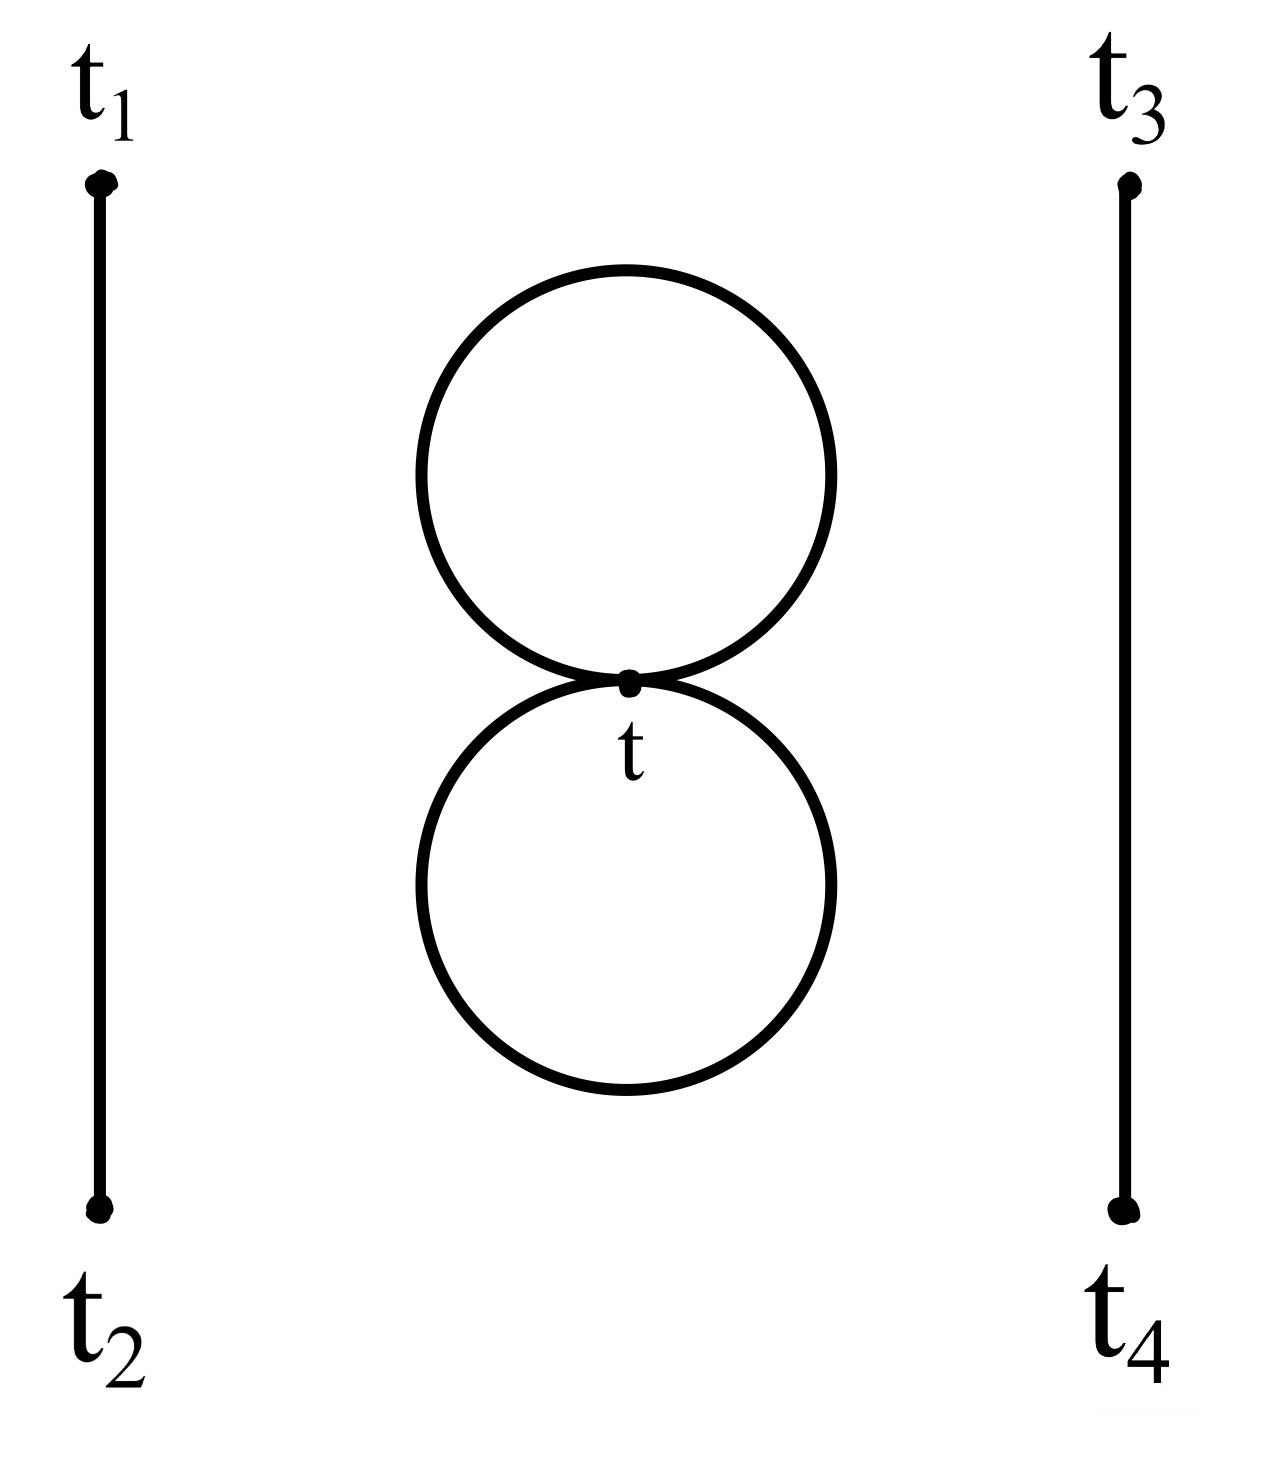
\includegraphics[width=5cm]{sections/IMG_1200.jpeg}
    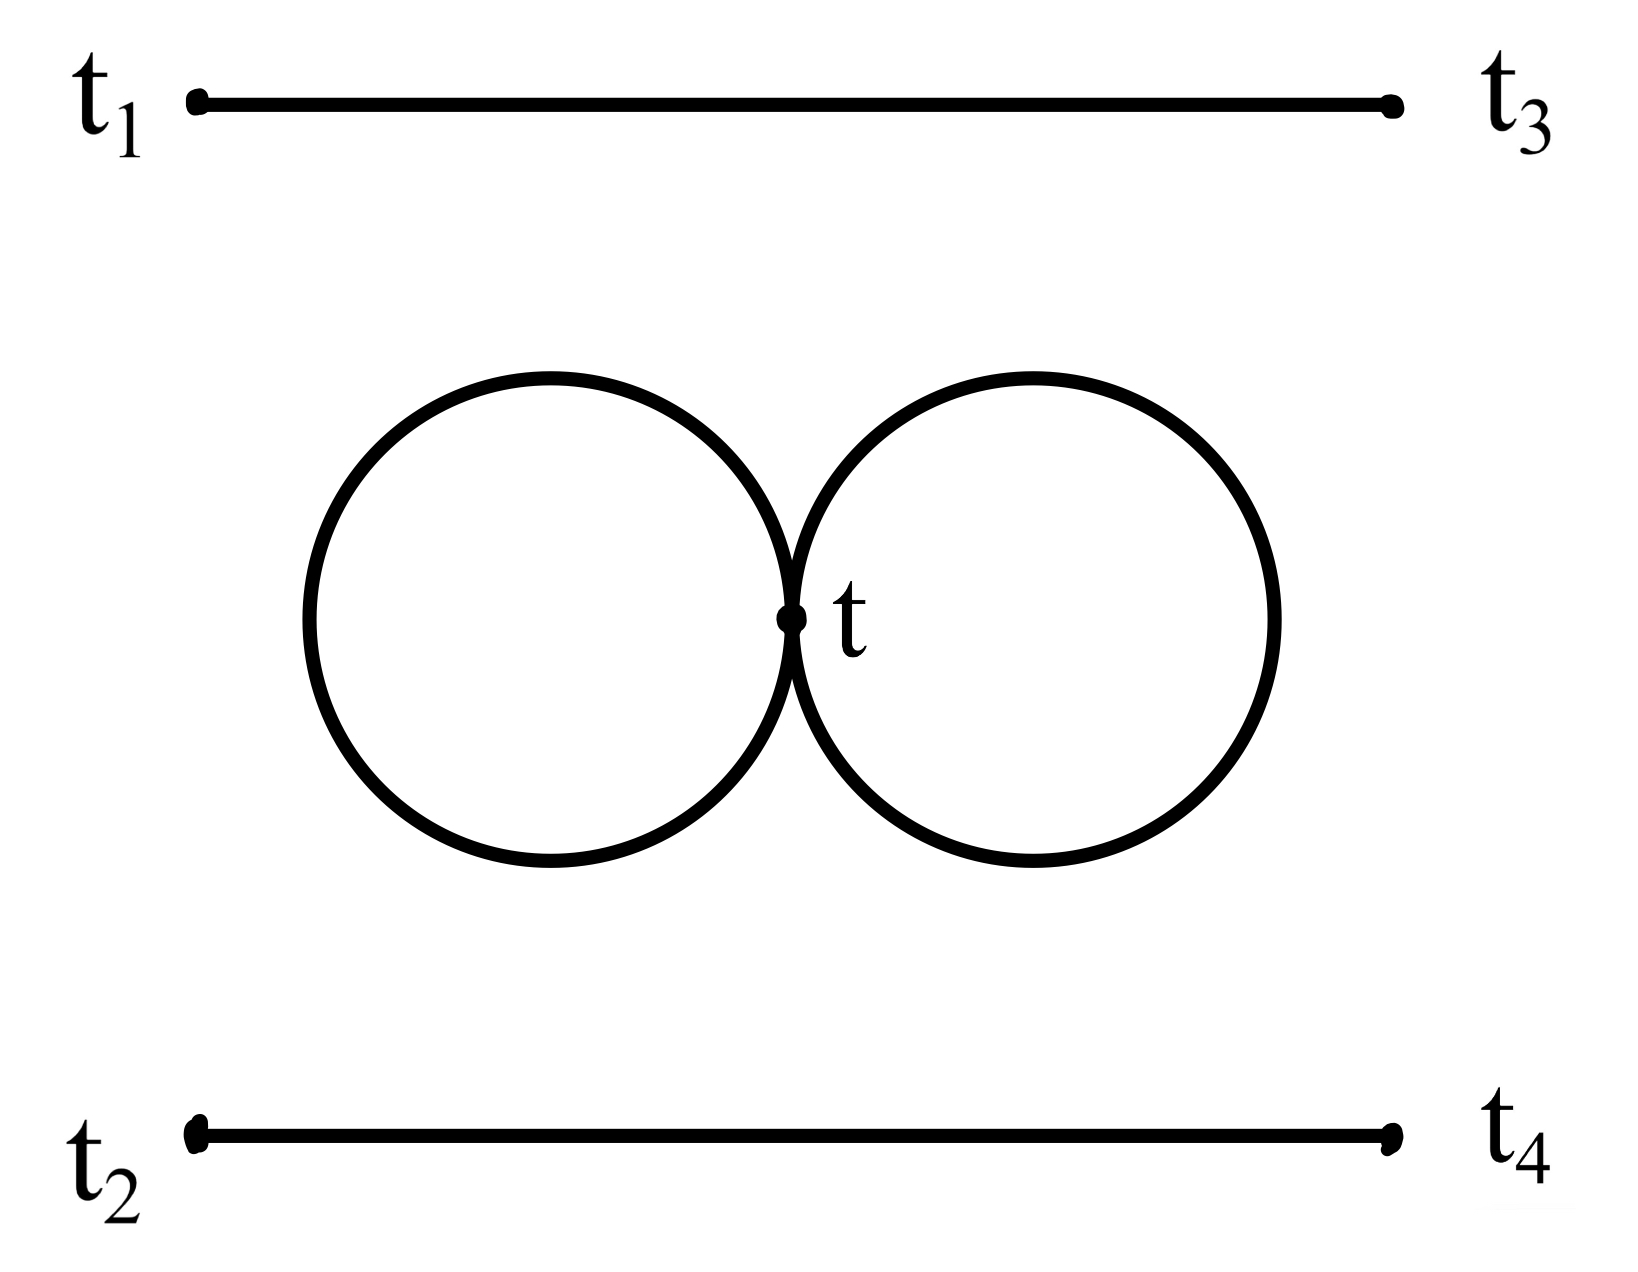
\includegraphics[width=5cm]{sections/IMG_1202.jpeg}
    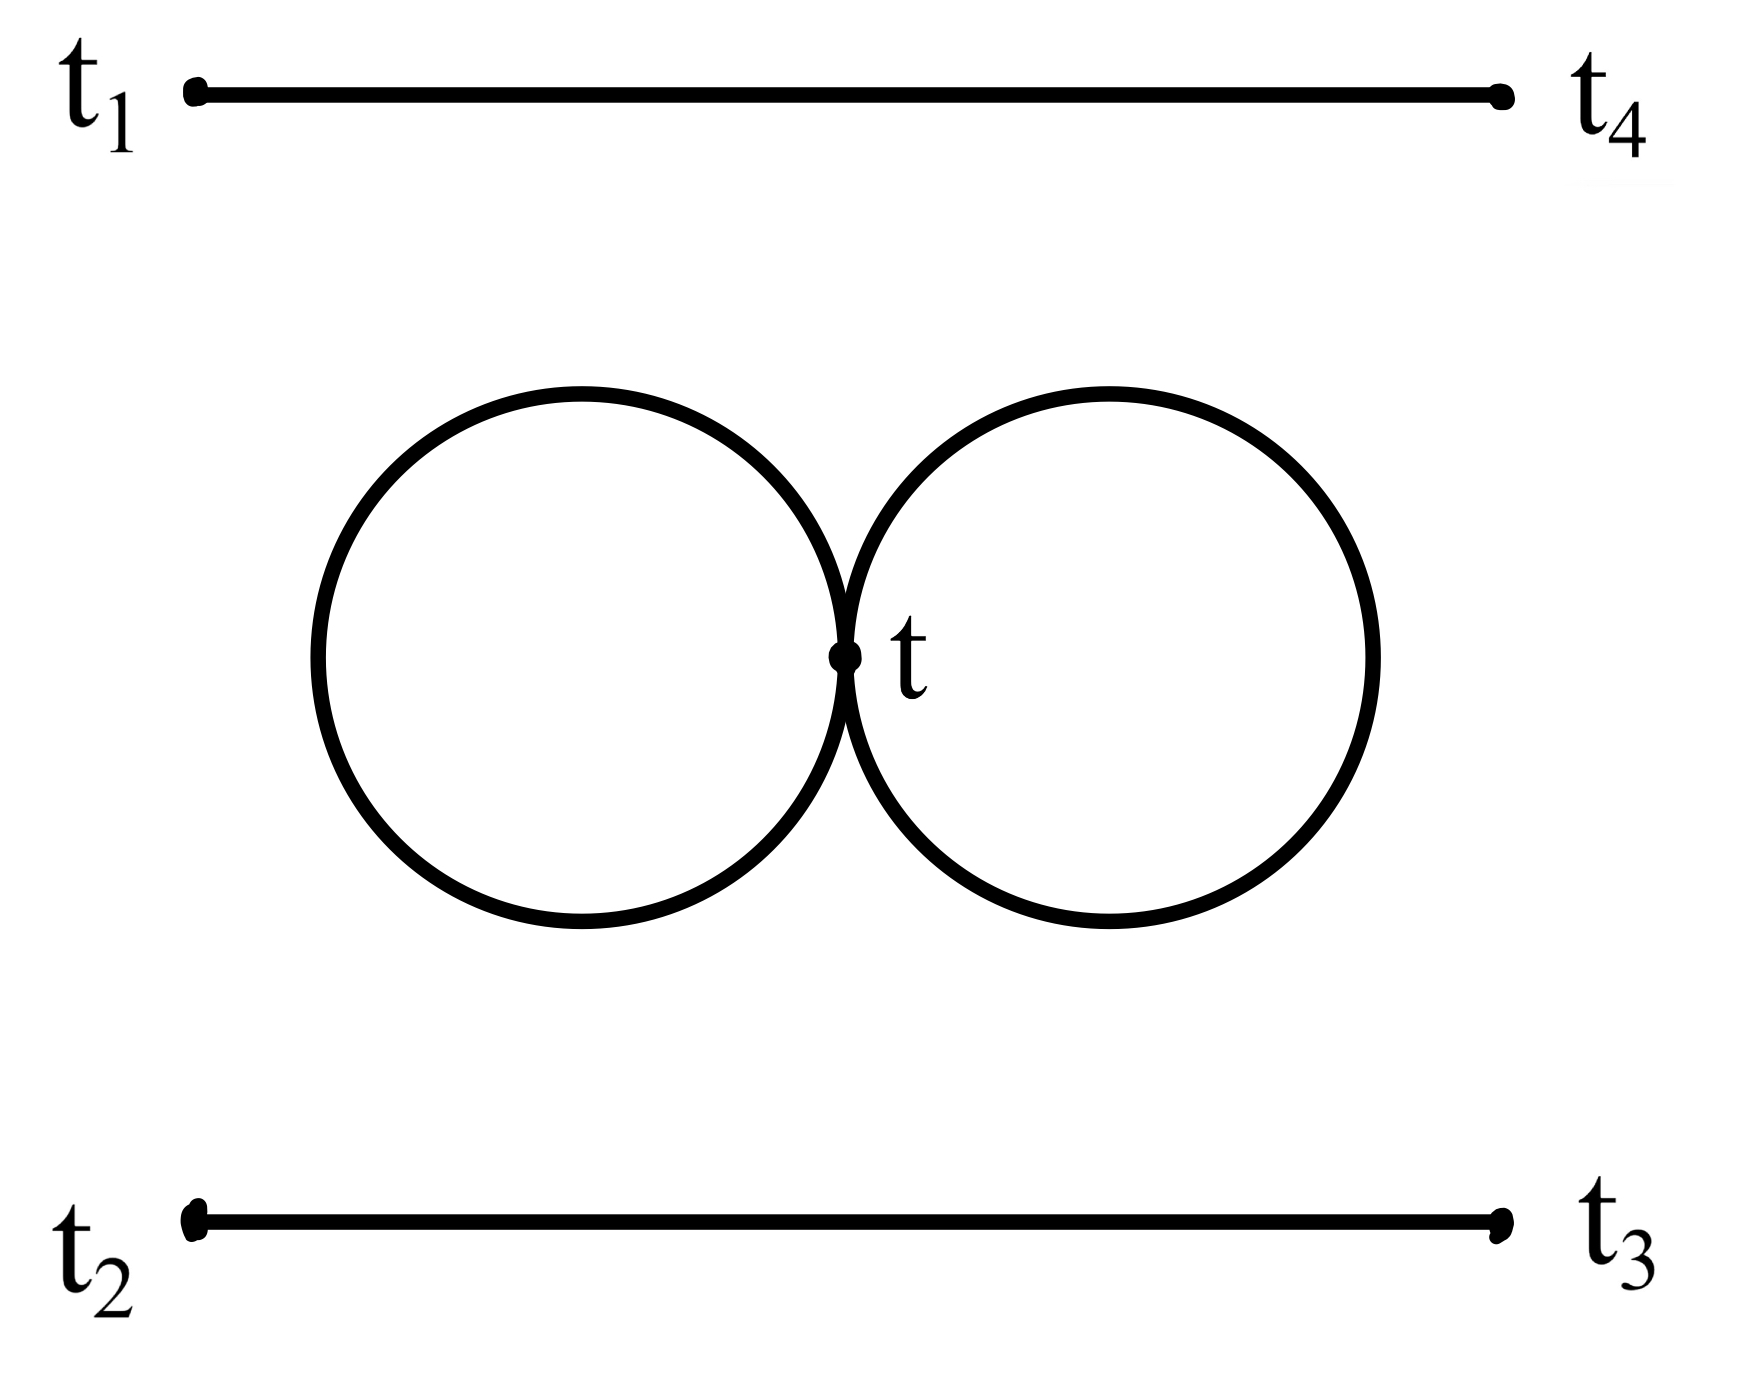
\includegraphics[width=5cm]{sections/IMG_1203.jpeg}
    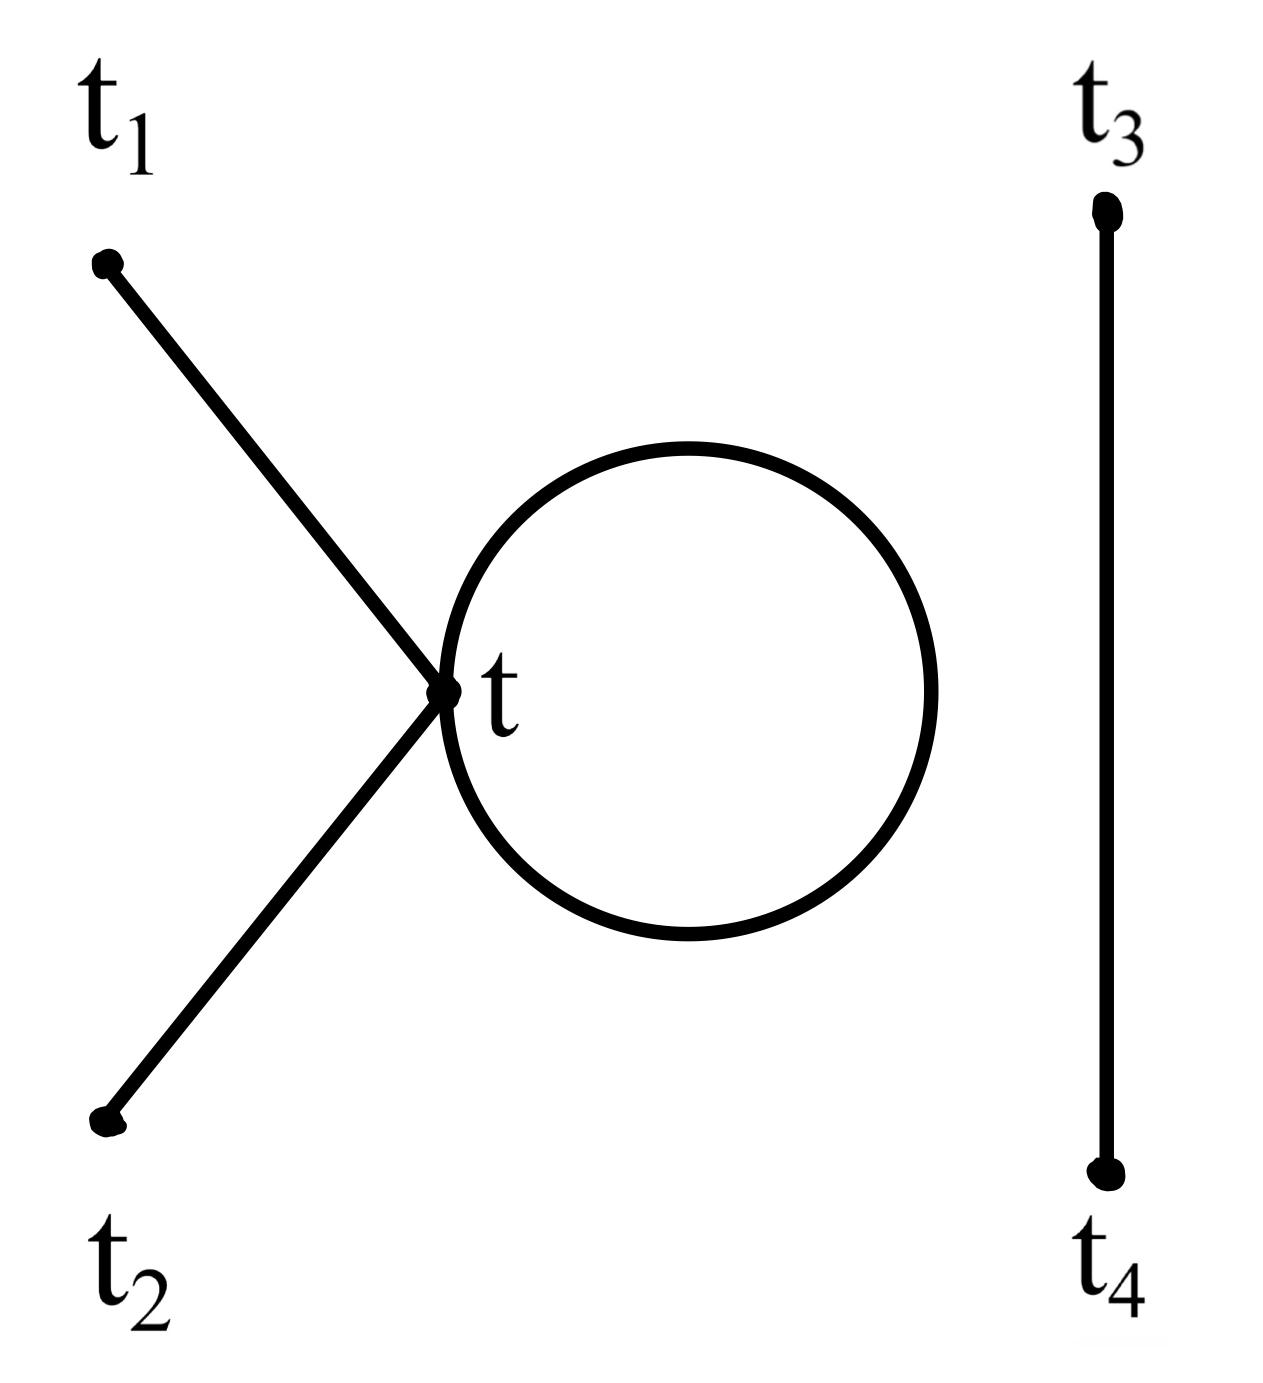
\includegraphics[width=5cm]{sections/IMG_1204.jpeg}
    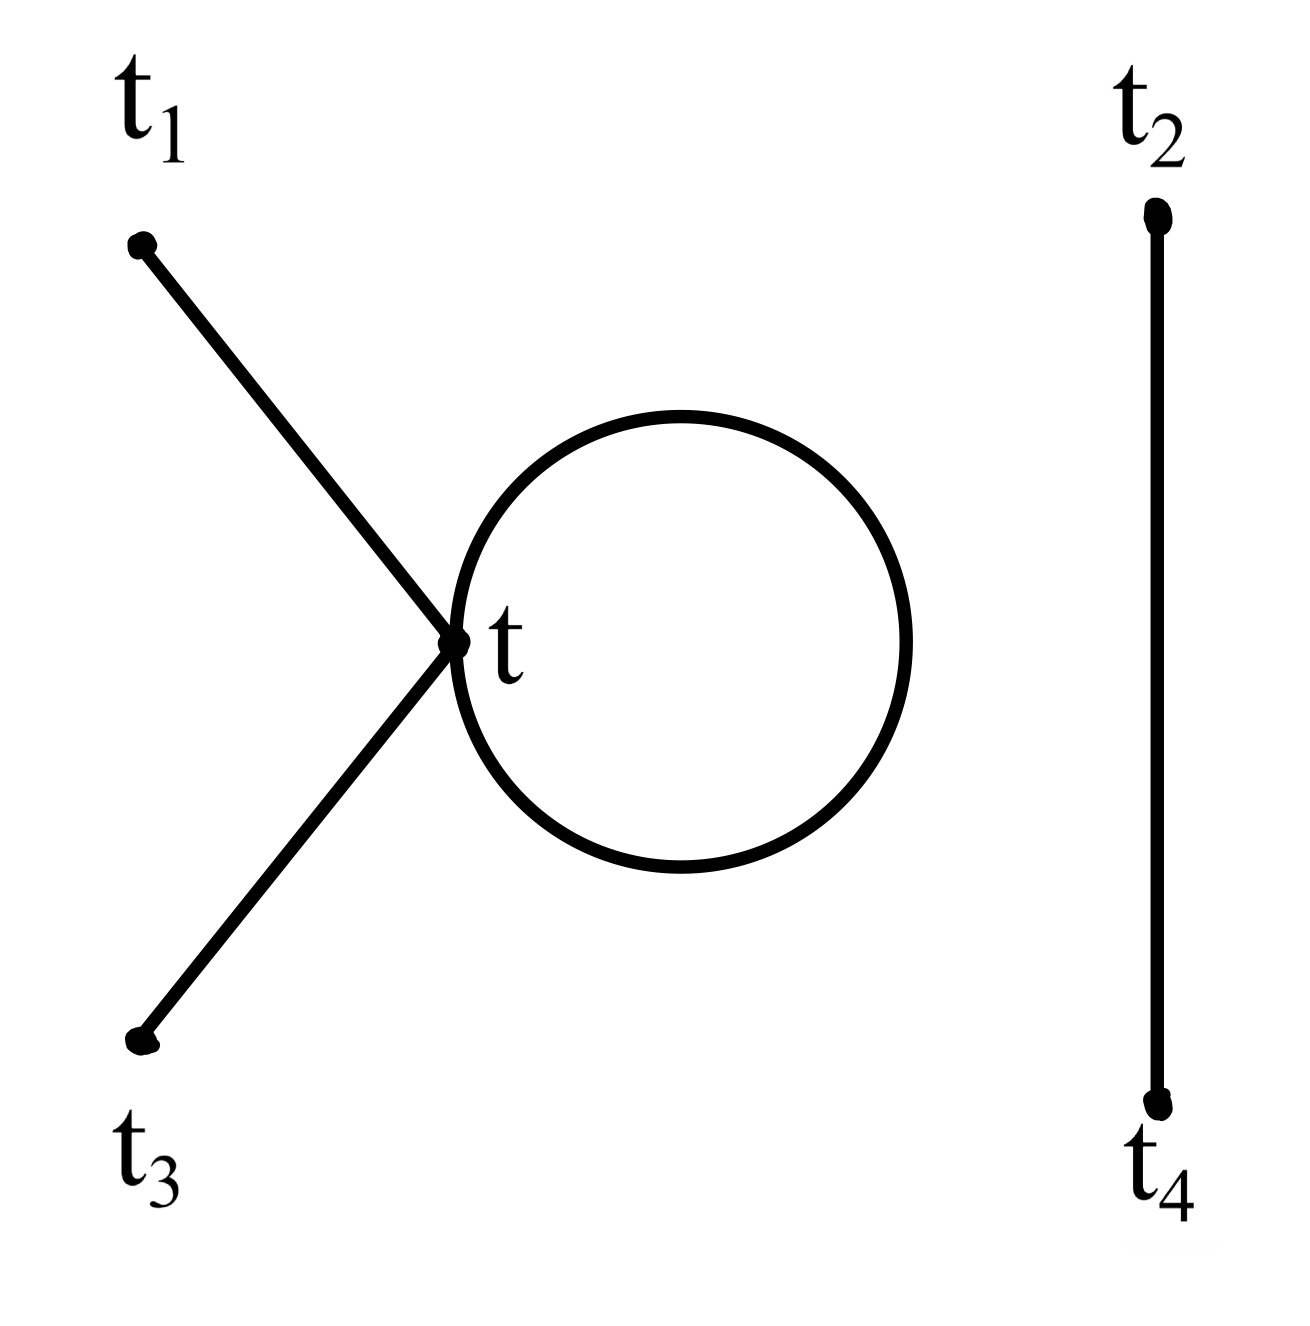
\includegraphics[width=5cm]{sections/IMG_1205.jpeg}
    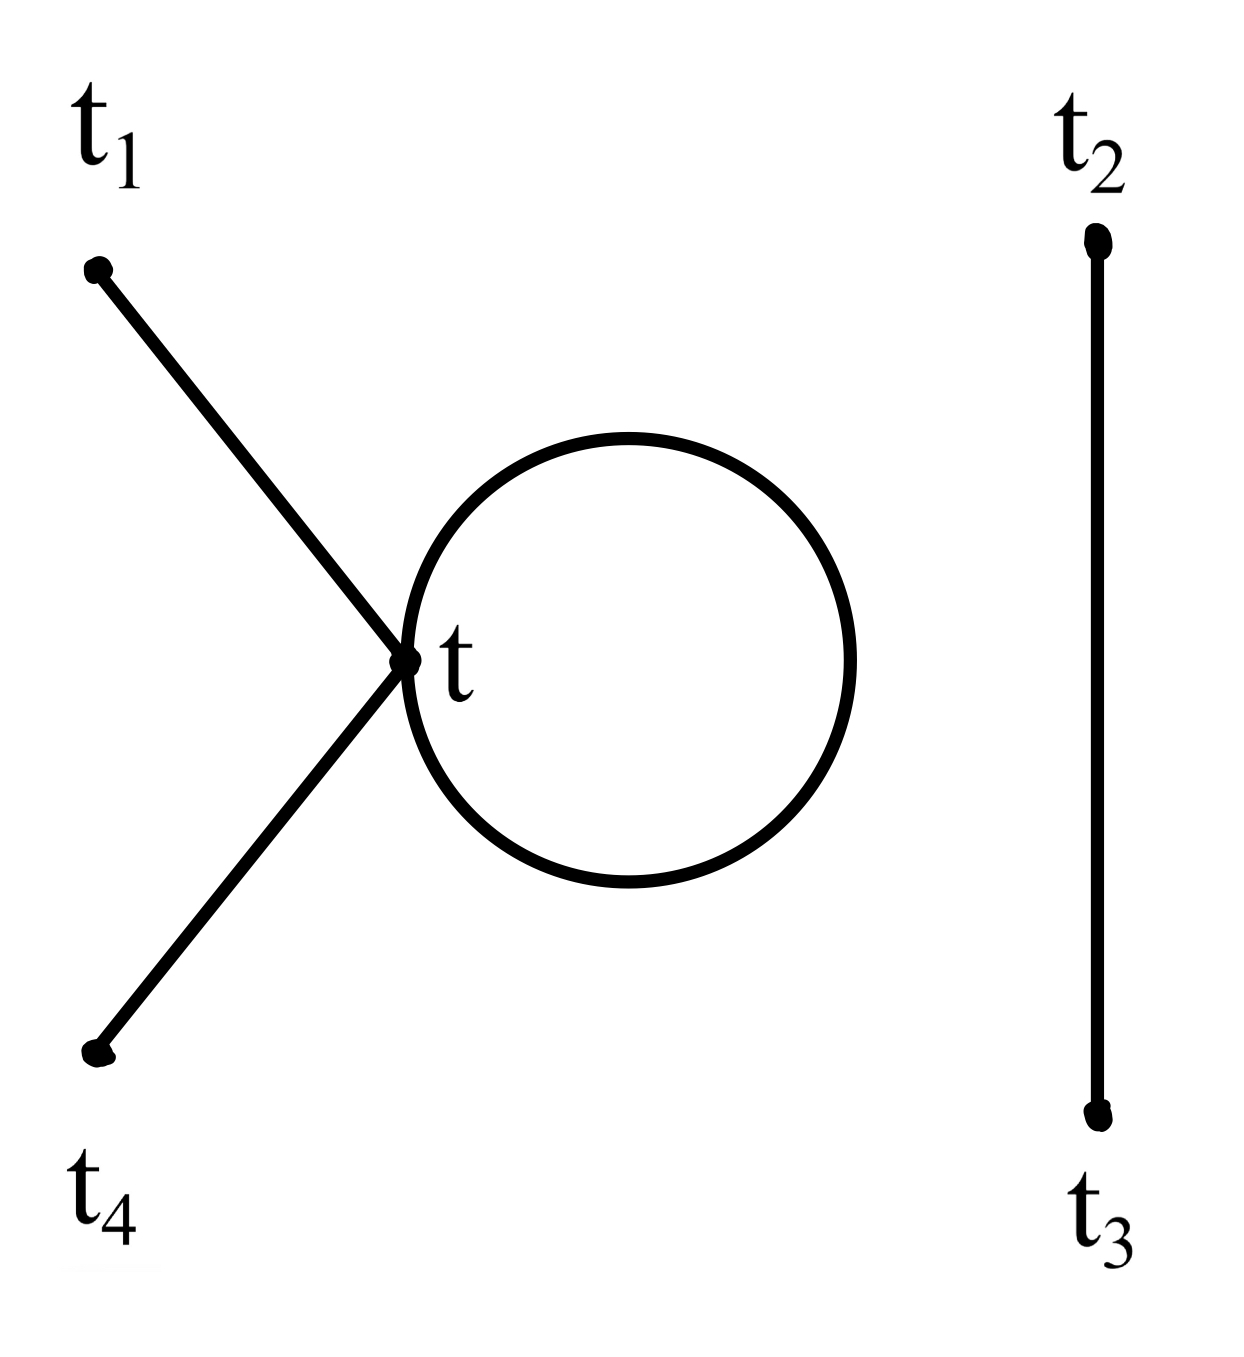
\includegraphics[width=5cm]{sections/IMG_1206.jpeg}
    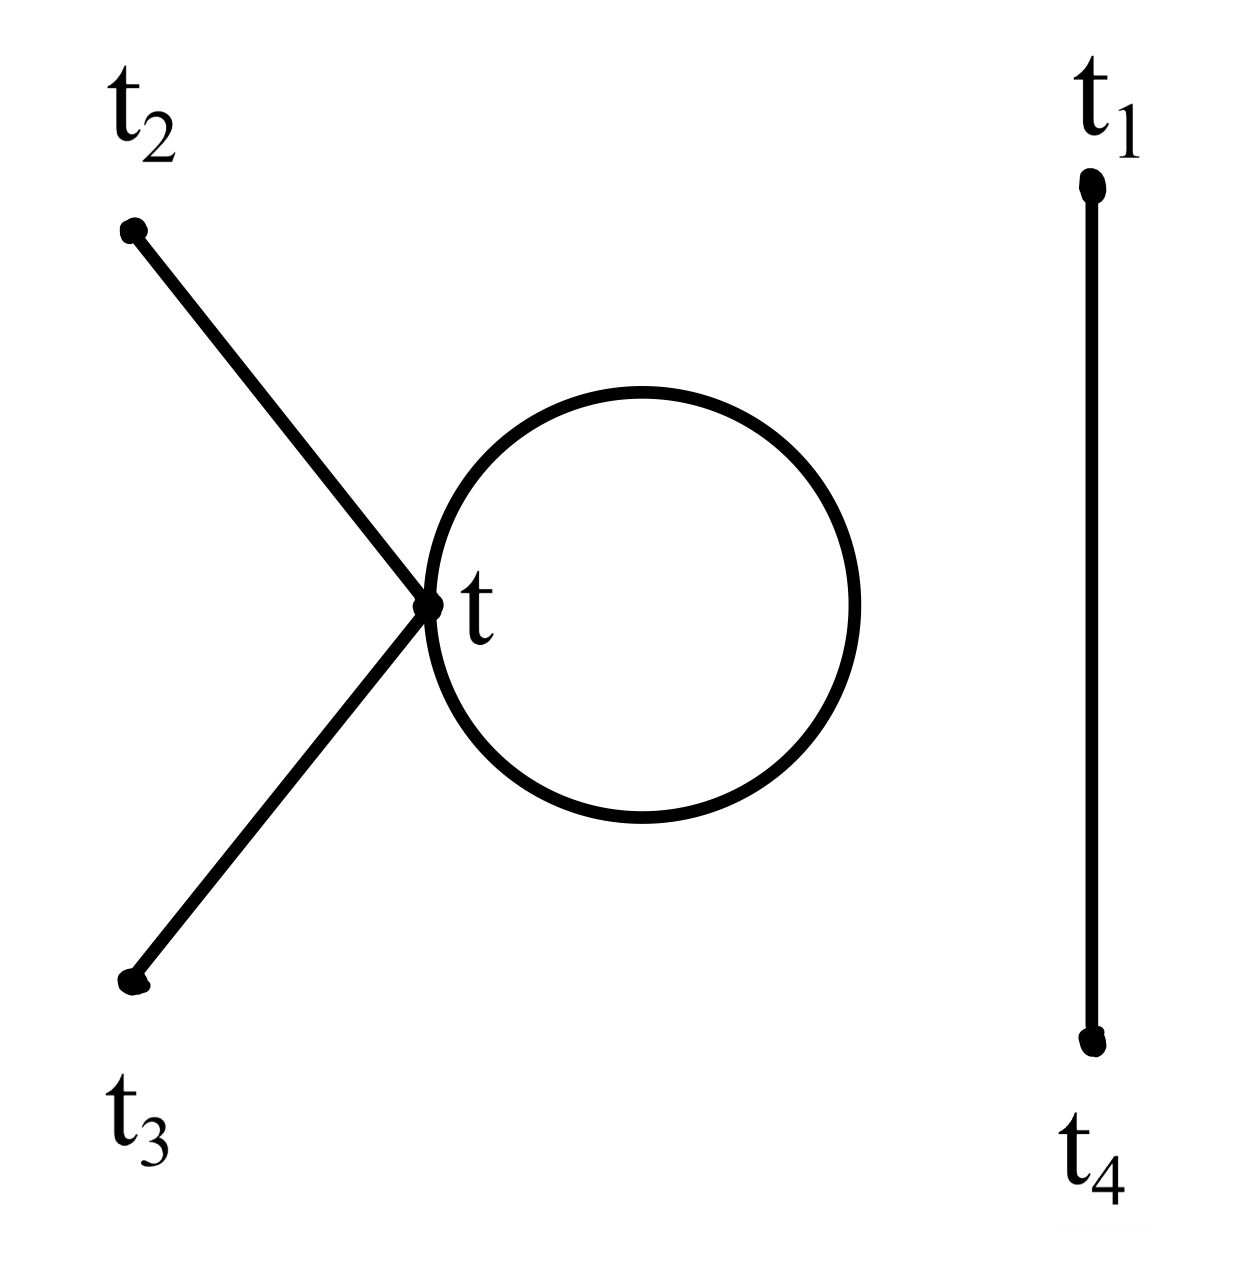
\includegraphics[width=5cm]{sections/IMG_1207.jpeg}
    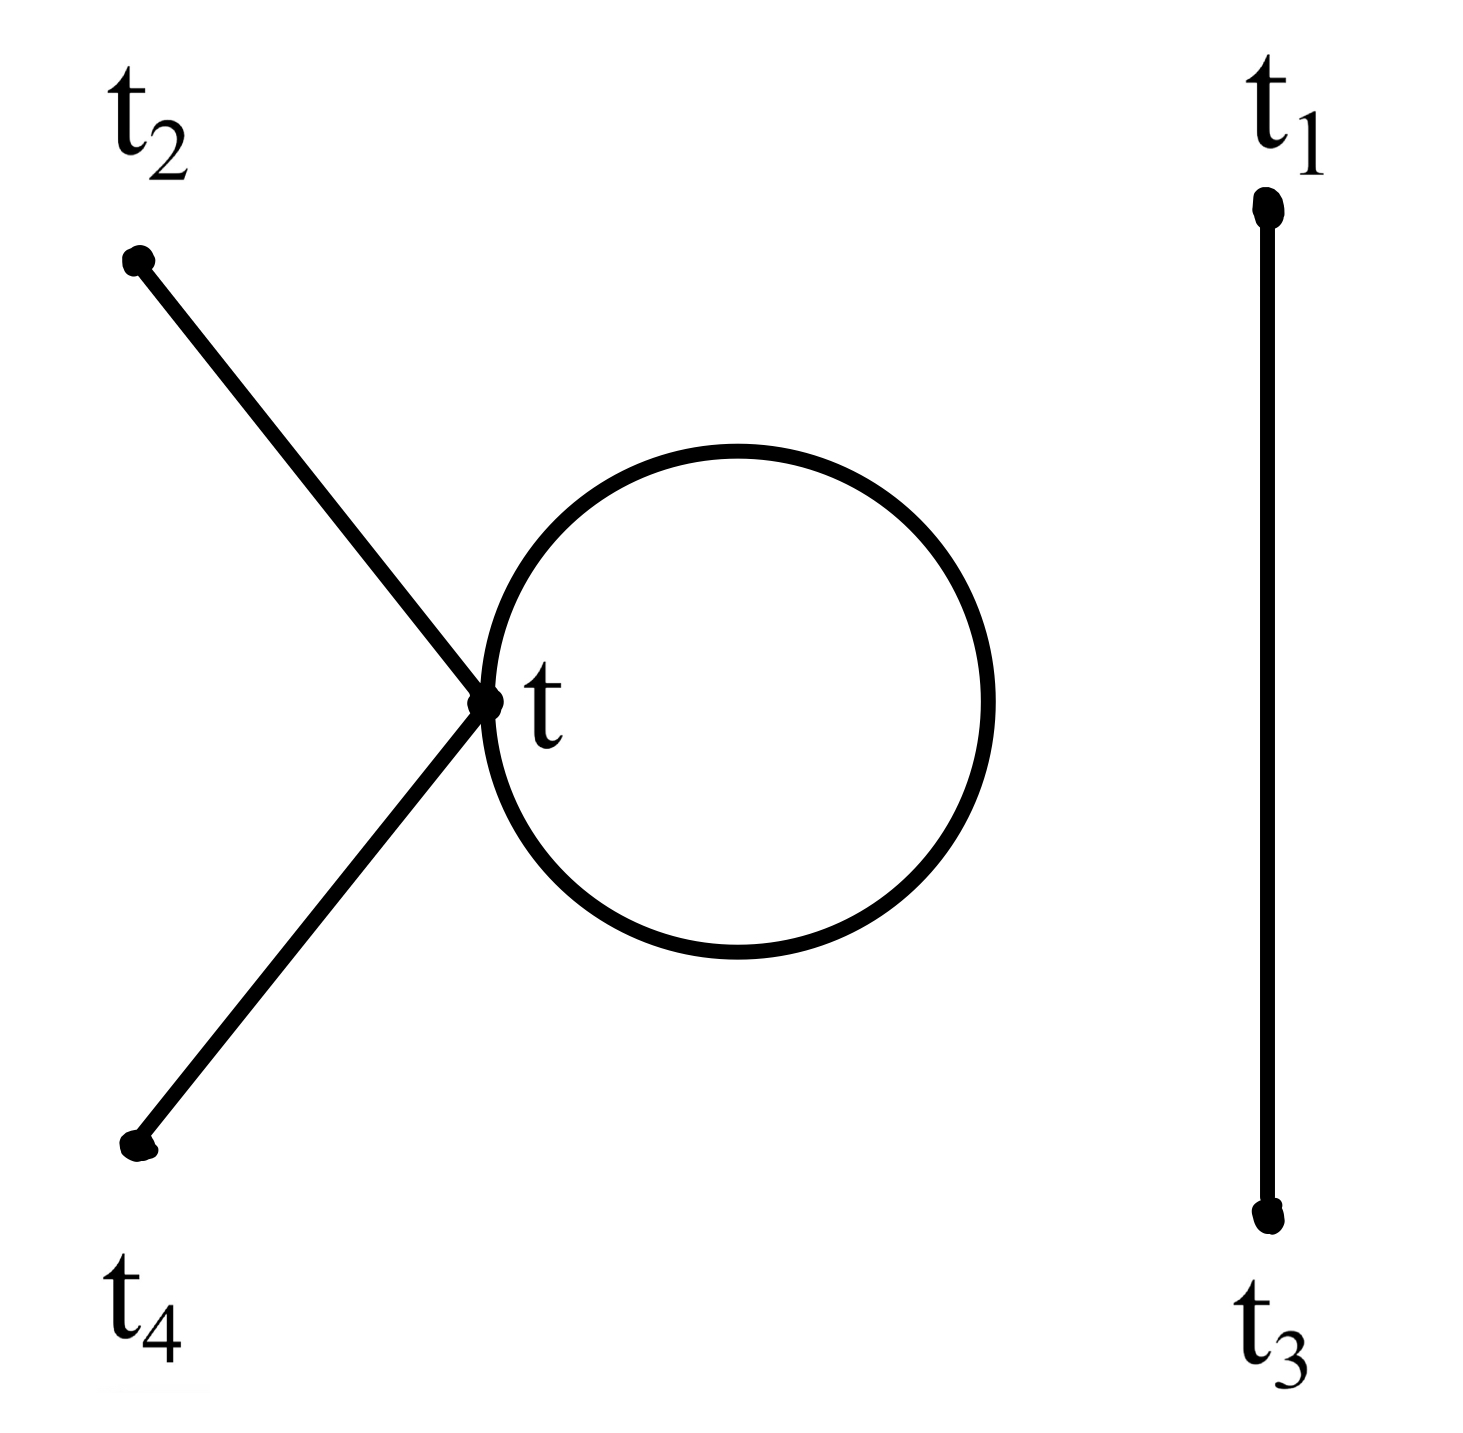
\includegraphics[width=5cm]{sections/IMG_1208.jpeg}
    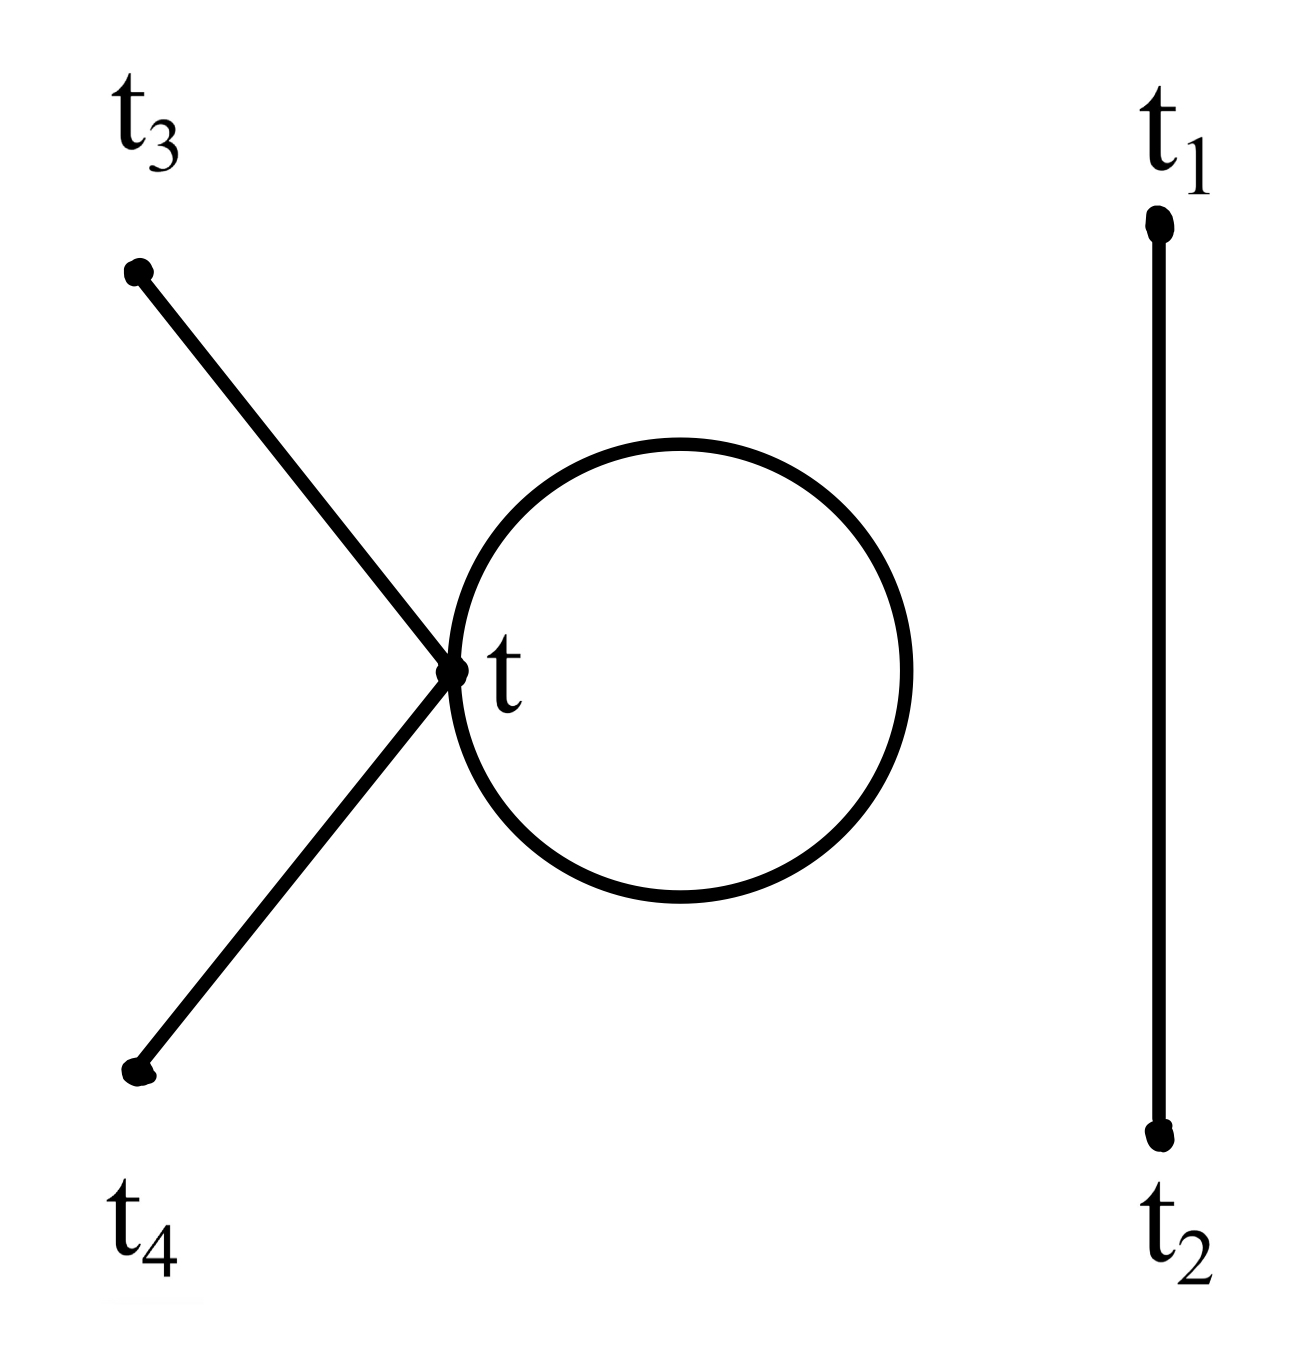
\includegraphics[width=5cm]{sections/IMG_1209.jpeg}
    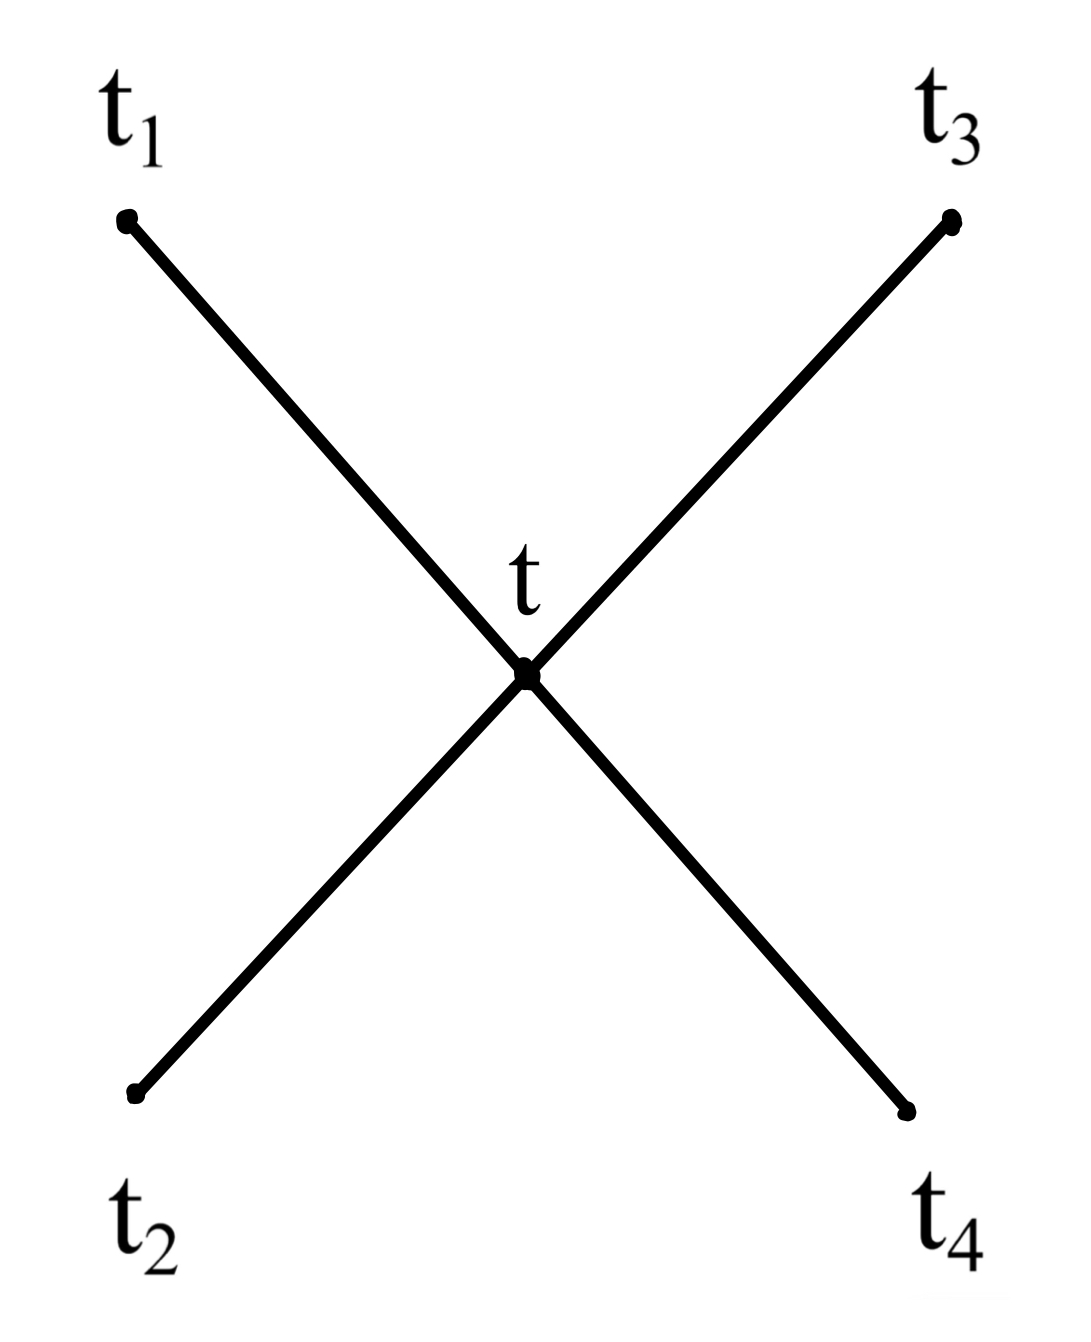
\includegraphics[width=5cm]{sections/IMG_1210.jpeg}
\end{center}
The integrals for the diagrams are given by 
\begin{align}
    D_1=-i\lambda \int dt G(t_1,t_2)G(t_3,t_4)G(t,t)G(t,t) \\
    D_2=-i\lambda \int dt G(t_1,t_3)G(t_2,t_4)G(t,t)G(t,t)\\
    D_3=-i\lambda \int dt G(t_1,t_4)G(t_2,t_3)G(t,t)G(t,t)\\
    D_4=-i\lambda \int dt G(t_1,t)G(t_2,t)G(t,t)G(t_3,t_4)\\
    D_5=-i\lambda \int dt G(t_1,t)G(t_3,t)G(t,t)G(t_2,t_4)\\
    D_6=-i\lambda \int dt G(t_1,t)G(t_4,t)G(t,t)G(t_2,t_3)\\
    D_7=-i\lambda \int dt G(t_2,t)G(t_3,t)G(t,t)G(t_1,t_4)\\
    D_8=-i\lambda \int dt G(t_2,t)G(t_4,t)G(t,t)G(t_1,t_3)\\
    D_9=-i\lambda \int dt G(t_3,t)G(t_4,t)G(t,t)G(t_1,t_2)\\ 
    D_{10}=-i\lambda \int dt G(t_1,t)G(t_2,t)G(t,t_3)G(t,t_4).
\end{align}
Thus, the total contribution of this term will be 
\begin{equation}
    \bra{0} T\{\hat x_I(t_1)\hat x_I(t_2)\hat x_I(t_3)\hat x_I(t_4)\left(-\frac{i\lambda}{4!}\right)\int_{-T}^T dt \hat x_I^4(t)\}\ket{0}=s_1(D_1+D_2+D_3)+s_2(D_4+...+D_9)+s_3D_{10}
\end{equation}
where the $s_i$ are the symmetry factors for each diagram. From the packet, we know $s_1=\frac 3 {4!}=\frac 1 8$. The diagrams $4...9$ all have 1 loop, so $s_2=\frac 2 {4!}=\frac 1 {12}$. The 10th diagram has no loops, so $s_3$ is simply $\frac 1 {4!}=\frac 1 {24}$.


\subsection{Exercise}
Inserting the factors from 9.2, we get 
\begin{align}
    \frac{\bra{0} T\{\hat x_I(t_1)\hat x_I(t_2)\hat x_I(t_3)\hat x_I(t_4)\}\ket{0}+\bra{0} T\{\hat x_I(t_1)\hat x_I(t_2)\hat x_I(t_3)\hat x_I(t_4)\left(-\frac{i\lambda}{4!}\right)\int_{-T}^T dt \hat x_I^4(t)\}\ket{0}}{1-\frac{i\lambda} 8 \int dt G(t,t)G(t,t)}\\
    =\frac{G_{12}G_{34}+G_{13}G_{24}+G_{14}G_{23}+s_1(D_1+D_2+D_3)+s_2(D_4+...+D_9)+s_3D_{10}}{1-\frac{i\lambda} 8 \int dt G(t,t)G(t,t)}.
\end{align}
Using the expansion
\begin{equation}
    \frac 1 {1-x}=1+x+x^2...
\end{equation}
and keeping terms first order in $\lambda$, we get (letting $s_1=\frac 1 8$ and plugging in the expressions for $D_1,D_2$, and $D_3$):
\begin{align}
    &(G_{12}G_{34}+G_{13}G_{24}+G_{14}G_{23}+s_1(D_1+D_2+D_3)+s_2(D_4+...+D_9)+s_3D_{10}...)(1+\frac{i\lambda} 8 \int dt G(t,t)G(t,t)...)\\&=G_{12}G_{34}+G_{13}G_{24}+G_{14}G_{23}\\&+(G_{12}G_{34}+G_{13}G_{24}+G_{14}G_{23})(\frac{i\lambda} 8 \int dt G(t,t)G(t,t))\\&-(G_{12}G_{34}+G_{13}G_{24}+G_{14}G_{23})(\frac{i\lambda} 8 \int dt G(t,t)G(t,t))+s_2(D_4+...+D_9)+s_3D_{10}).
\end{align}
Noting that the second and third terms cancel, we are left with
\begin{equation}
    G_{12}G_{34}+G_{13}G_{24}+G_{14}G_{23}+s_2(D_4+...+D_9)+s_3D_{10}.
\end{equation}

\subsection{Exercise}
The integral for this diagram is
\begin{equation}
    -i\lambda \int_{-T}^TdtG(t_1,t)G(t_2,t)G(t,t).
\end{equation}
Using the Green's function for a harmonic oscillator, 
\begin{equation}
    G(t_2,t_1)=\frac 1 {2\omega} e^{-i\omega |t_2-t_1|},
\end{equation}
this is 
\begin{equation}
    -i\lambda\int_{-T}^T \frac {dt}{(2\omega)^3}e^{-i\omega(|t_1-t|+|t_2-t|+|t-t|)}. 
\end{equation}
Inserting $t_1=t_2=0$, this simplifies to 
\begin{equation}
     -i\lambda \int_{-T}^T \frac{dt}{(2\omega)^3} e^{-2\omega i |t|}=-\frac{i\lambda}{(2\omega^3)}\left[2\int_0^T dt e^{-2\omega i t}\right]
\end{equation}
because the integrand is even in $t$. This integral can be evaluated as
\begin{equation}
    -\frac{i\lambda}{(2\omega)^3}\frac 2 {-2\omega i}\left[e^{-2\omega i T}-1\right]= -\frac{2\lambda}{(2\omega)^4}\left[1-e^{-2\omega i T}\right].
\end{equation}
In the limit $T \to \infty (1 - i\epsilon)$, the second term becomes
\begin{equation}
    \lim_{T \to \infty (1 - i\epsilon)}e^{-2\omega i T}=e^{-2\omega i \infty}e^{-2\omega \epsilon \infty}=0
\end{equation}
when $\epsilon>0$, and since the first term always has magnitude 1. Then the diagram evaluates to 
\begin{equation}
    -\frac{2\lambda}{(2\omega)^4}=-\frac{\lambda}{8\omega^4}.
\end{equation}
\bibliographystyle{plain}
\bibliography{bib.bib}
\end{document}
